% !TEX root=../main.tex

\chapter{Active and sterile neutrinos}
\label{chap:theory_introduction}

\dictum[Richard P. Feynman]{
    It doesn't matter how beautiful your theory is, it doesn't matter how smart you are. 
    If it doesn't agree with experiment, it's wrong.
}

\section{Neutrinos: a journey across history}

Dating back to 1914, the history of neutrinos began with the first paper published by Sir James Chadwick \cite{chadwickIntensityDistributionMagnetic1914}, who, investigating the phenomenology of beta decays, discovered that the emitted electron energy spectra was not a single vertical emission line (delta shaped) but a continuous spectrum. 

The $\beta$ decay process, up until then, was thought to be just the emission of a single electron from a neutron decaying at rest to a proton, $\Pn \to \Pp + \Pem,$ and so the electron was expected to carry all the neutron energy. A continuous $\Pem$ spectrum broke this expectation. W. Pauli in 1930 proposed the idea that the emission of the electron occurred along with the emission of another fermionic particle, far less massive --- massless even --- than the electron, carrying no electric charge \cite{pauliDearRadioactiveLadies1978}. Even if Pauli did not label this particle ``neutrino'' yet, its idea was all contained in his letter.

Enrico Fermi, a prominent scientist of that era, developed Pauli's idea, calling this new particle \emph{neutrino} \cite{fermiTentativoDiTeoria1934, fermiVersuchTheorieVStrahlen1934} --- from \emph{neutron}, the only chargeless particle discovered so far, aside from photons --- adding the suffix \emph{-ino}, meaning smaller (and lighter). Fermi's idea was the first \emph{field theory} of quantum mechanics, suggesting that the $\beta$ decay could be formalized as a four-fermion point interaction, involving a neutron decaying to a proton to produce an electron and a neutrino, \begin{equation}
    \beta^-: \quad \Pn \to \Pp + \Pem + \PAGne. \implies 
    \feynmandiagram[baseline=(current bounding box.center), horizontal=a to b, scale=0.85]{
        a [particle=$\PAGne$] -- [fermion] e,
        c [particle=$\Pn$] -- [fermion] e,
        e -- [fermion] b [particle=$\Pp$],
        e -- [fermion] d [particle=$\Pem$] 
    };
    \label{eq:fermi_4p}
\end{equation}

Fermi's effective theory managed to explain the $\beta$ decay energy spectrum of the electron successfully, even preserving the angular momentum conservation. The value of the coupling constant measured by Fermi for this interaction, called $G_F$, was \begin{equation}
    G_F^{(\beta)} \simeq \SI{1.166e-5}{\per\giga\electronvolt\squared}, 
\end{equation} implying that this type of interaction had a minimal cross section, which justified calling this type of interaction \emph{weak}. Up until then, however, the neutrino was yet to be ``directly'' observed. It took twenty-six years of experimental efforts to actually detect the traces of this ``ghostly'' particle. The first experimental observation of electron antineutrinos produced by beta decays from the Savannah River reactor happened in 1956; a team led by F. Reines and C. L. Cowan observed the signature of inverse beta decay process (IB) \begin{equation}
    \PAGne + \Pp \to \Pn + \Pep
\end{equation} in a water tank. The positron quickly finds an electron in water and produces two gamma rays by pair annihilation. This does not provide a unique signature, since there are other processes producing two gamma rays in water. So the complete event signature required the additional detection of the neutron. Using cadmium --- a strong neutron absorber --- dissolved in water, photons from the de-excitation of cadmium were detected, a mere \SI{5}{\us} after the prompt photons from IBD \cite{cowanDetectionFreeNeutrino1956}. 

The world of particle physics was discovering new particles very fast and putting together the picture we today know as the Standard Model (SM) of particle physics: in the same years the electron neutrino was discovered, a team led by Carl D. Anderson and Seth Neddermeyer discovered the muon by detecting charged particles with weather balloons at different heights in the atmosphere, which they described as the heavier relative to the electron, since it showed a less prominent curvature than the electron when passed through a magnetic field; this discovery was later confirmed \cite{andersonCloudChamberObservations1936, neddermeyerNoteNatureCosmicRay1937, streetNewEvidenceExistence1937}. 
The discovery led many physicists to start questioning the relationship between neutrinos and muons/electrons.
In 1959 Bruno Pontecorvo examined this problem and questioned himself about the nature of neutrinos \cite{pontecorvoElectronMuonNeutrinos1991}: are neutrinos produced alongside electrons and neutrinos produced alongside muons the same? This led to the neutrino experiment at Brookhaven National Laboratories (BNL) guided by L. M. Lederman, M. Schwarz, and J. Steinberger. At BNL, using the Brookhaven Alternating Gradient Synchrotron (AGS), protons were accelerated toward a beryllium target: the resulting kaons and pions decayed in-flight, producing muons and muon antineutrinos.  Using a spark chamber located behind a concrete wall stopping the produced muons, they were able to detect the muons produced by the interaction of muon antineutrinos but saw no electron-like event. This represented strong proof that there are at least two \emph{families} of neutrinos \cite{PhysRevLett.9.36}.  

In 1989 the ALEPH detector at the LEP $\Pep\Pem$ collider studied the $\PZz$ resonance and set strong constraints on the number of neutrino families $N_\PGn \simeq 3$ \cite{decampPreciseDeterminationNumber1990}, thereby ruling out the possibility of a fourth (active) neutrino family and suggesting a third neutrino should exist. In 1975 the third ``\emph{heavier}'' brother of the electron and the muon, the tau, was discovered \cite{perlEvidenceAnomalousLepton1975}; this discovery led physicists to expect that a third neutrino had to exist. The tau neutrino signature was finally detected in 2000 in the DONuT (Direct Observation of the Nu Tau) experiment at Fermilab, twenty-five years after the discovery of the tau lepton. 

\section{Neutrinos in the Standard Model}

The state of the art of particle physics is defined by the Standard Model (SM). 
In the SM of particle physics the strong, weak and electromagnetic interactions are described by the gauge symmetries $\mathrm{SU(3)_C\times SU(2)_L \times U(1)_Y}$ \cite{peskinIntroductionQuantumField1995}.  The SM is the most comprehensive theory of particle physics, and has been experimentally tested with high accuracy. 
Neutrinos in the minimal SM are massless fermions --- meaning that their spin is half-integer --- that do not have strong nor electromagnetic interactions. As for all the particles in the SM, we can define the helicity $\mathcal H = \boldsymbol{\sigma} \cdot \vb p / \qty|\vb p|$ as the projection of the spin $\boldsymbol{\sigma}$ on the particle momentum $\vb p$; however, differently from other particles of the SM, for neutrinos only left-handed ($\mathcal H = -1$) neutrinos and right-handed ($\mathcal H = +1$) neutrinos have been observed. 
The experimental evidence of this peculiarity of neutrinos was first seen by M. Goldhaber, L. Grodzins and A. W. Sunyar in 1958 \cite{goldhaberHelicityNeutrinos1958}.
Helicity for massless particles is equivalent to their chirality (or handedness), which is why we can define positive helicity as right-handed neutrinos and negative helicity as left-handed neutrinos. 

The SM includes three families of neutrinos, each paired with the corresponding charged lepton: the electron neutrino $\PGne$, the muon neutrino $\PGnGm$ and the tau neutrino $\PGnGt$, and the corresponding three antiparticles. 

\subsection{Neutrino interactions}

In the SM neutrinos can, therefore, only interact via the weak interaction, which is mediated by three vector bosons, $\PWpm$ and $\PZz$. The experimental evidence of the $\PWpm$ and $\PZz$ bosons, constituting a strong proof of the SM theory, arrived between 1982 and 1983. The experiments UA1/UA2, led by Nobel physics laureate Carlo Rubbia, and located inside the CERN-S$\Pp\PAp$S accelerator ring, saw signatures of these bosons with proton-antiproton collisions with a high significance \cite{arnisonExperimentalObservationLepton1983, bannerObservationSingleIsolated1983a}. 

% some details of the type of interactions in the SM
The types of interactions that are possible for neutrinos are multiple. In general a neutrino can interact with other SM particles via the exchange of either a $\PW$ boson --- thus resulting in a charged current (CC) event, with the corresponding charged lepton on the other side of such vertices --- or of a $\PZ$ boson --- resulting in a neutral current (NC) interaction, where the outgoing particle is the same flavour neutrino. In both cases, the diagram is completed by stitching on the other side of the boson line the interaction with the matter. The interaction in its entirety is required to conserve both charge and momentum. 
According to what the final state particles of the interaction are, the interactions themselves can be classified. 
A brief description of the most relevant interaction modes is provided in the following.

%% CC interaction

\begin{figure}
    \centering
    \subfloat[]{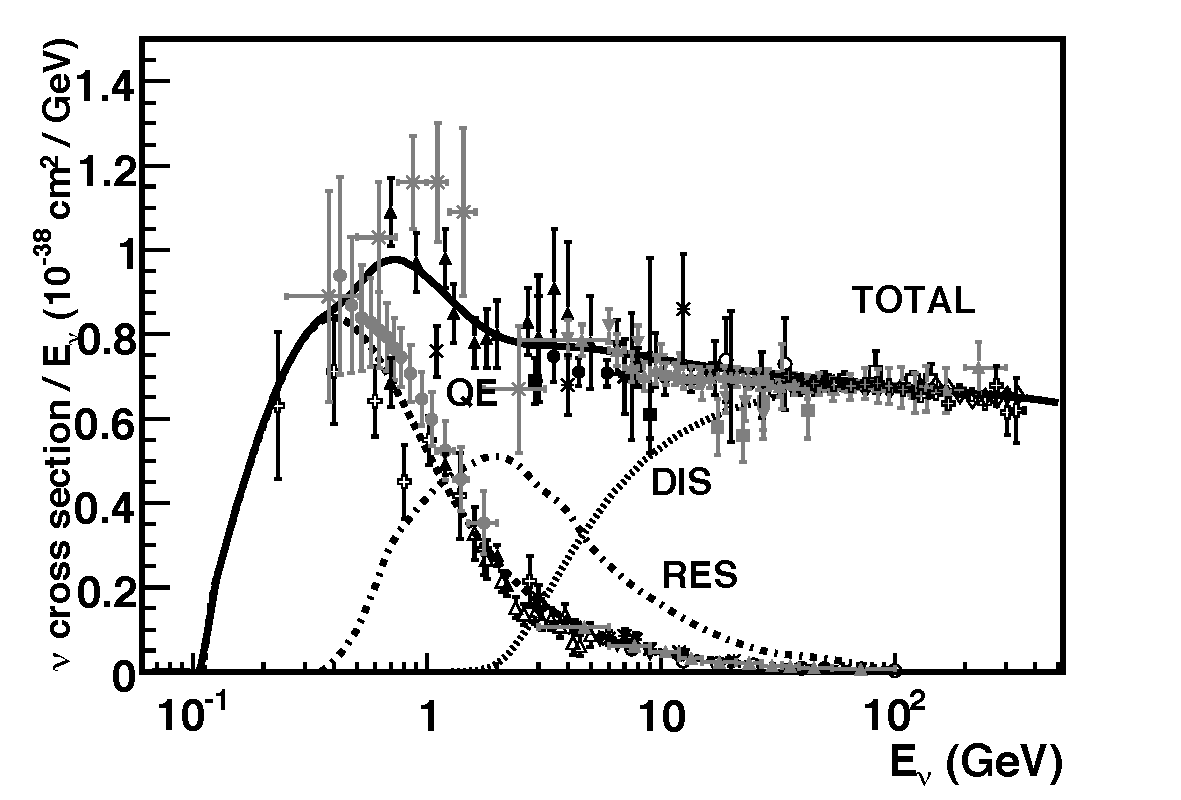
\includegraphics[width=0.95\linewidth, trim={0 0.5cm 0 0.5cm}]{theory/cc_inclusive_nu.pdf}\label{fig:xs_nu}}
    
    \subfloat[]{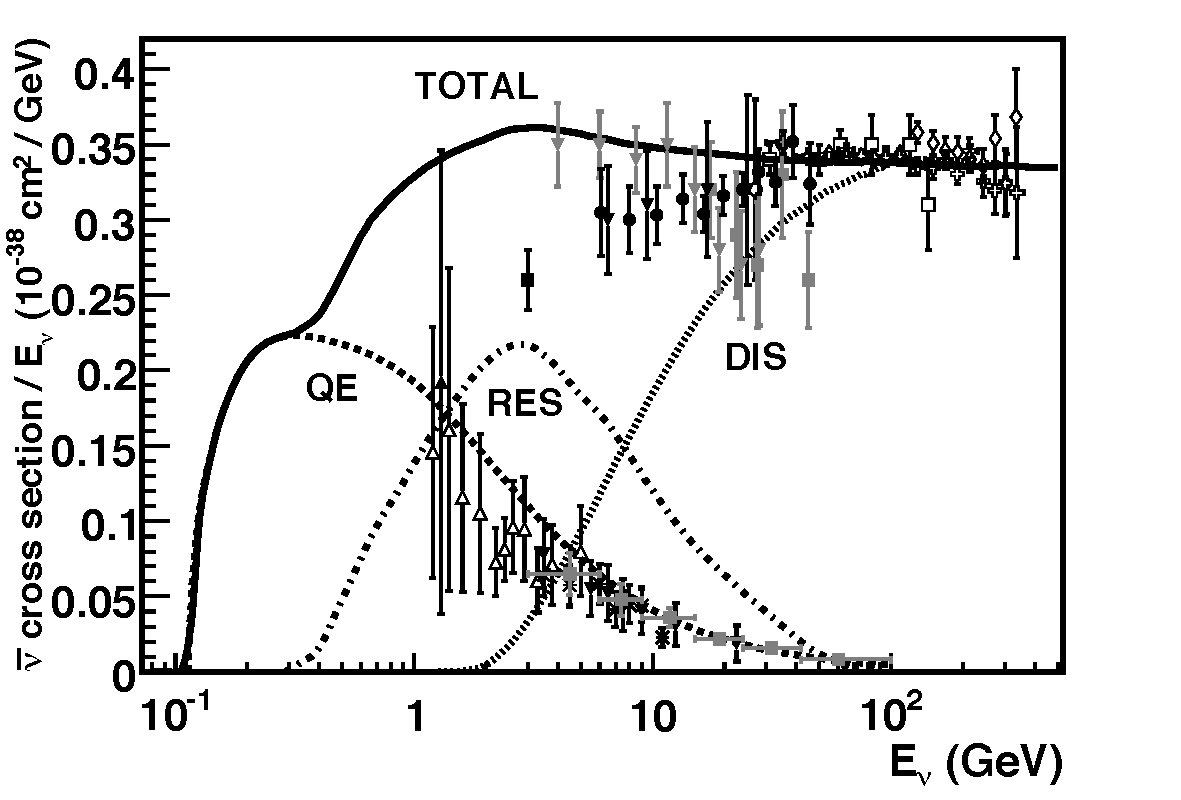
\includegraphics[width=0.95\linewidth, trim={0 0.5cm 0 0.5cm}]{theory/cc_inclusive_nubar.pdf}\label{fig:xs_nubar}}
    \caption[(Anti)Neutrino-matter cross-sections]{Cross-section measurements for (anti)neutrino-nucleon charged current interactions, showing the contributions of quasi-elastic, resonant, and deep-inelastic-scattering processes, both for neutrinos \ref{sub@fig:xs_nu} and for antineutrinos \ref{sub@fig:xs_nubar}. Figures adapted from Ref. \cite{formaggioEVEeVNeutrino2012}.}
    \label{fig:xs_both}
\end{figure}

\begin{figure}
    \centering

    \subfloat[CC QE]{
        \begin{tikzpicture}
            \begin{feynman}
                \vertex (numu) {$\PGnGm$};
                \vertex[right=3cm of numu] (mu) {$\PGm$};
                \vertex[below right=.75cm and 1.5cm of numu] (v0);
                \vertex[blob, below right=1.cm and .75cm of v0] (v1) {};
                \vertex[below left=.75cm and 1.5cm of v1] (neutron) {$\Pn$};
                \vertex[below right=.75cm and 1.5cm of v1] (proton) {$\Pp$}; 
    
                \diagram*{
                    (numu) -- [fermion] (v0) -- [fermion] (mu),
                    (v0) -- [boson, edge label'=$\PWp$] (v1),
                    (neutron) -- [fermion] (v1) -- [fermion] (proton)
                };
            \end{feynman}
        \end{tikzpicture}
        \label{fig:interaction_CCQE}
    }\hspace{4em}
    \subfloat[NC El.]{
        \begin{tikzpicture}
            \begin{feynman}
                \vertex (numu) {$\PGnGm$};
                \vertex[right=3cm of numu] (mu) {$\PGnGm$};
                \vertex[below right=.75cm and 1.5cm of numu] (v0);
                \vertex[blob, below right=1.cm and .75cm of v0] (v1) {};
                \vertex[below left=.75cm and 1.5cm of v1] (neutron) {$\Pp$};
                \vertex[below right=.75cm and 1.5cm of v1] (proton) {$\Pp$}; 
    
                \diagram*{
                    (numu) -- [fermion] (v0) -- [fermion] (mu),
                    (v0) -- [boson, edge label'=$\PZz$] (v1),
                    (neutron) -- [fermion] (v1) -- [fermion] (proton)
                };
            \end{feynman}
        \end{tikzpicture}
        \label{fig:interaction_NCEl}
    }

    \subfloat[CC Res.]{
        \begin{tikzpicture}
            \begin{feynman}
                \vertex (numu) {$\PGnGm$};
                \vertex[right=3cm of numu] (mu) {$\PGm$};
                \vertex[below right=.75cm and 1.5cm of numu] (v0);
                \vertex[blob, below right=1.cm and .75cm of v0] (v1) {};
                \vertex[below left=.75cm and 1.5cm of v1] (neutron) {$\Pp$};
                \vertex[below right=.25cm and 1.25cm of v1] (DELTA1);
                \vertex[above right=.5cm and 1.cm of DELTA1] (pi) {$\PGpp$};
                \vertex[below right=.5cm and 1.cm of DELTA1] (proton) {$\Pp$};
    
                \diagram*{
                    (numu) -- [fermion] (v0) -- [fermion] (mu),
                    (v0) -- [boson, edge label'=$\PWp$] (v1),
                    (neutron) -- [fermion] (v1) -- [fermion, edge label=$\PGDpp$] (DELTA1),
                    (DELTA1) -- [fermion] (pi),
                    (DELTA1) -- [fermion] (proton)
                };
            \end{feynman}
        \end{tikzpicture}
        \label{fig:interaction_CCRes}
    }\hspace{2em}
    \subfloat[NC Res.]{
        \begin{tikzpicture}
            \begin{feynman}
                \vertex (numu) {$\PGnGm$};
                \vertex[right=3cm of numu] (mu) {$\PGnGm$};
                \vertex[below right=.75cm and 1.5cm of numu] (v0);
                \vertex[blob, below right=1.cm and .75cm of v0] (v1) {};
                \vertex[below left=.75cm and 1.5cm of v1] (neutron) {$\Pp$};
                \vertex[below right=.25cm and 1.25cm of v1] (DELTA1);
                \vertex[above right=.5cm and 1.cm of DELTA1] (pi) {$\PGpp$};
                \vertex[below right=.5cm and 1.cm of DELTA1] (proton) {$\Pn$};
    
                \diagram*{
                    (numu) -- [fermion] (v0) -- [fermion] (mu),
                    (v0) -- [boson, edge label'=$\PZz$] (v1),
                    (neutron) -- [fermion] (v1) -- [fermion, edge label=$\PGDp$] (DELTA1),
                    (DELTA1) -- [fermion] (pi),
                    (DELTA1) -- [fermion] (proton)
                };
            \end{feynman}
        \end{tikzpicture}
        \label{fig:interaction_NCRes}
    }

    \subfloat[CC DIS]{
        \begin{tikzpicture}
            \begin{feynman}
                \vertex (numu) {$\PGnGm$};
                \vertex[right=3cm of numu] (mu) {$\PGm$};
                \vertex[below right=.75cm and 1.5cm of numu] (v0);
                \vertex[blob, below right=1.cm and .75cm of v0] (v1) {};
                \vertex[below left=.75cm and 1.5cm of v1] (neutron) {$N^{(0)}$};
                \vertex[below right=.5cm and 1.45cm of v1] (p0); 
                \vertex[below right=.25cm and 1.5cm of v1] (p1); 
                \vertex[right=2.cm of v1] (p2) {$X^{(+)}$}; 
                \vertex[above right=.25cm and 1.5cm of v1] (p3); 
                \vertex[above right=.5cm and 1.45cm of v1] (p4);
    
                \diagram*{
                    (numu) -- [fermion] (v0) -- [fermion] (mu),
                    (v0) -- [boson, edge label'=$\PWp$] (v1),
                    (neutron) -- [fermion] (v1) -- {(p0), (p1), (p2), (p3), (p4)}
                };
            \end{feynman}
        \end{tikzpicture}
        \label{fig:interaction_CCDIS}
    }\hspace{4em}
    \subfloat[NC DIS]{
        \begin{tikzpicture}
            \begin{feynman}
                \vertex (numu) {$\PGnGm$};
                \vertex[right=3cm of numu] (mu) {$\PGnGm$};
                \vertex[below right=.75cm and 1.5cm of numu] (v0);
                \vertex[blob, below right=1.cm and .75cm of v0] (v1) {};
                \vertex[below left=.75cm and 1.5cm of v1] (neutron) {$N^{(0)}$};
                \vertex[below right=.5cm and 1.45cm of v1] (p0); 
                \vertex[below right=.25cm and 1.5cm of v1] (p1); 
                \vertex[right=2.025cm of v1] (p2) {$Y^{(0)}$}; 
                \vertex[above right=.25cm and 1.5cm of v1] (p3); 
                \vertex[above right=.5cm and 1.45cm of v1] (p4); 
    
                \diagram*{
                    (numu) -- [fermion] (v0) -- [fermion] (mu),
                    (v0) -- [boson, edge label'=$\PZz$] (v1),
                    (neutron) -- [fermion] (v1) -- {(p0), (p1), (p2), (p3), (p4)}
                };
            \end{feynman}
        \end{tikzpicture}
        \label{fig:interaction_NCDIS}
    }
    
    \caption{Diagrams of some interaction topologies for neutrinos in matter}
    \label{fig:interactions}
\end{figure}

% \begin{figure}
%     \[
%         \begin{tikzpicture}[baseline=(current bounding box.center)]
%             \begin{feynman}
%                 \vertex (numu) {$\PGnGm$};
%                 \vertex[right=3cm of numu] (mu) {$\PGm$};
%                 \vertex[below right=.75cm and 1.5cm of numu] (v0);
%                 \vertex[blob, below right=1.5cm and .75cm of v0] (v1) {};
%                 \vertex[below left=.75cm and 1.5cm of v1] (neutron) {$\Pn$};
%                 \vertex[below right=.75cm and 1.5cm of v1] (proton) {$\Pp$}; 
    
%                 \diagram*{
%                     (numu) -- [fermion] (v0) -- [fermion] (mu),
%                     (v0) -- [boson, edge label=$\PW$] (v1),
%                     (neutron) -- [fermion] (v1) -- [fermion] (proton)
%                 };
%             \end{feynman}
%         \end{tikzpicture}
%         \qquad\overset{q^2 \ll s}{\looongrightarrow} \qquad
%         \feynmandiagram[baseline=(current bounding box.center), horizontal=a to b, scale=0.75]{
%             a [particle=$\Pn$] -- [fermion] e,
%             c [particle=$\PGne$] -- [fermion] e,
%             e -- [fermion] b [particle=$\Pp$],
%             e -- [fermion] d [particle=$\Pem$] 
%         };
%     \]
%     \caption[The link between the Fermi four-fermion interaction and the SM diagrams]{The effect of integrating out the massive boson in the $\beta$ decay process. Neither the proton, nor the neutron are ``elementary'' particles, so their interaction with the $\PW$ boson is not as straight forward, hence the ``blob'' shape replacing the interaction vertex.}
%     \label{fig:SM2fermi}
% \end{figure}

\paragraph{Charged current interactions} Neutrino-matter interactions show a rich phenomenology that varies dramatically across different energy scales. Multiple mechanisms determine the total cross-section of the $\PGn$-matter interaction, as shown by \autoref{fig:xs_both}. \begin{itemize}
    \item Starting on the lower part of the energy spectrum, the first mechanism we encounter is the so-called quasielastic interaction. This mechanism has an energy peak around $E_\PGn\simeq \mathcal O (\SI{1}{GeV})$. In a QE event, the neutrino scatters off an entire nucleon rather than its constituent partons, converting the neutron to a proton and emitting a charged lepton \begin{equation}
        \PGn_\ell + \Pn \to \ell^- + \Pp, \quad \PAGn_\ell + \Pp \to \ell^+ + \Pn.
    \end{equation} The diagrams corresponding to such processes are shown in Figure \ref{fig:interaction_CCQE}. The QE neutrino cross-section can be accurately described by the V-A interaction theory, being an effective theory between the Fermi four-point interaction and the SM \cite{formaggioEVEeVNeutrino2012}.

    \item As we approach $E_\PGn \simeq \mathcal O (\SI{10}{GeV})$, neutrinos can excite the struck nucleon to an excited state. In this case, the neutrino interaction produces a baryon resonance, which in most cases quickly decays to a nucleon and single pion final state, as illustrated in figure \ref{fig:interaction_CCRes}, where the following resonance pion production process is pictured \begin{equation}
        \PGn_\ell + p \overset{\PGDpp}{\looongrightarrow} \ell^- + \PGpp + \Pp.
    \end{equation} In addition to resonance production, neutrinos can also coherently produce single pion final states. In this case, the neutrino coherently scatters from the entire nucleus, transferring negligible energy to the target. These low-$Q^2$ interactions produce no nuclear recoil and a distinctly forward-scattered pion, compared to their resonance-mediated counterparts.

    \item When the neutrino energy exceeds \SI{10}{GeV}, the interaction is entirely at the parton level \cite{formaggioEVEeVNeutrino2012}, breaking the nucleons and producing a final state interaction with high multiplicity, i.e. a large number of final state particles, \begin{equation}
        \PGn_\ell + N^{(0)} \to \ell^- + X^{(+)}, \quad \PAGn_\ell + N^{(0)} \to \ell^+ + X^{(-)}
    \end{equation} where $X^{(\pm)}$ indicates the ensemble of the final state particles, with this notation highlighting that charge is still conserved, so an overall positive charge is expected. This kind of interaction is known as Deep Inelastic Scattering (DIS) \cite{formaggioEVEeVNeutrino2012}. This is exemplified in Figure \ref{fig:interaction_CCDIS}. 
\end{itemize}

%% NC interaction (and Gargamelle!)
\paragraph{Neutral current interactions} The possible interactions include neutral current topologies mediated by the exchange of a $\PZz$ boson. Looking at the classification for CC events, we also have a similar classification for neutral current (NC) topologies. \begin{itemize}
    \item The lower part of the energy spectrum is populated by elastic scattering of neutrinos on nucleons, with each particle involved in the process not changing its nature, \begin{equation}
        \brabar{\PGn_\ell} + N \to \ell^\pm + N, \quad \text{with $N = \Pp, \Pn$}.
    \end{equation} One of these processes is presented in Figure \ref{fig:interaction_NCEl}.

    \item NC Resonance (Res.) and Coherent (Coh.) single pion scattering processes are also possible, with a plethora of possible final state topologies; in Figure \ref{fig:interaction_NCRes} as an example the single pion process mediated by the $\PGDp$ baryon is shown \begin{equation}
        \PGnGm + \Pp \overset{\PGDp}{\looongrightarrow} \PGnGm + \PGpp + \Pn.
    \end{equation}

    \item Finally, at high energy, the NC Deep Inelastic Scattering (DIS) processes are possible. Figure \ref{fig:interaction_NCDIS} shows an illustration of a DIS process, $\PGnGm + N^{(0)} \to \PGnGm + Y^{(0)}$. 
\end{itemize}

The Gargamelle experiment \cite{mussetNeutrinoPhysicsGargamelle1978} played a key role in the history of neutrino physics, being the first to actively detect signatures of neutral weak current events, thus confirming the validity of the weak interaction model \cite{hasertObservationNeutrinolikeInteractions1973, hasertSearchElasticMuonneutrino1973}. 
Full reviews of the neutrino interactions in matter (expanding more on the processes displayed in \autoref{fig:interactions}) are found in Ref. \cite{atharNeutrinosTheirInteractions2022, formaggioEVEeVNeutrino2012}. 

\subsection{Flavour oscillations}

Neutrinos are one of the most abundant ``visible'' particles in the universe. They are produced in multiple channels, many \emph{natural}, some \emph{artificial}. The production mechanism is correlated with their energy. \begin{itemize}
    \item Neutrinos in the MeV scale are generated in reactions inside the stars cores (such as the Sun) through the $\Pp\Pp$p-chain and the CNO cycle reactions \cite{agostiniExperimentalEvidenceNeutrinos2020};
    \item On the artificial side, neutrinos in the MeV region are those coming from nuclear fission reactors: electron antineutrinos originate as the $\beta$-decay products of unstable isotopes such as $^{238}$U and $^{239}$Pu. The energies peak at \SI{3}{MeV} and extend up to \SI{8}{MeV} \cite{Giunti:2021kab}; 
    \item The central part of the energy spectrum, from some GeV to some \si{TeV}, is composed of atmospheric neutrinos, coming from cosmic rays interacting within the atmosphere. These also compose the highest part of the spectrum;
    \item In the core region, there are also accelerator-borne beams of neutrinos. These extend from some hundreds of MeV to some tens of GeV and constitute an interesting part of the spectrum: their power can be controlled, hence their flux, making it easier to study in greater detail the properties of neutrinos.
\end{itemize}
Up to this point, the description of neutrinos has been of massless neutral leptons. However, experimental observations suggested otherwise. 

Dating back to the discovery of neutral mesons, the idea of flavour oscillation was established for massive particles. This was the case for the $\PKz/\PAKz$ system oscillation, which was studied to get an explanation for the regeneration of short-lived neutral kaons, $\PKzS$ \cite{landeReportLongLived$K^0$1957}. This type of oscillatory behaviour is accurately explained by the weak interaction of quarks in the SM Lagrangian with the Higgs mechanism that gives masses to quarks themselves, hence to mesons. $\PKz/\PAKz$ are both eigenstates of the weak interaction, which are different from the mass eigenstates that control the time evolution of the particle. When looking at the time evolution of the eigenstate of the weak interaction, we get, thus, an oscillatory behaviour. 

For neutrinos, based on experimental evidence, no flavour oscillation was expected. However, theoretical models of neutrino oscillation date back to the '60s. In 1957 Pontecorvo discussed $\PGmp\Pem \leftrightarrow \PGmm\Pep$ \cite{pontecorvoMesoniumAntimesonium1957}, and proposed, with an analogy to the $\PKz/\PAKz$ system, the oscillation of neutrinos. The two-flavour neutrino oscillation physics was worked out by Maki, Nakagawa and Sakata in 1962 \cite{makiRemarksUnifiedModel1962}. In this model, the oscillation probability is found to be proportional to \begin{equation}
    P(\PGn_\alpha \to \PGn_\beta) = \sin[2](2\theta_{\alpha\beta}) \sin[2](\frac{\Delta m^2 E_\PGn}{4L}),
\end{equation} where the probability of going from the flavour state $\alpha$ to the flavour state $\beta$ is dependent on the mixing angle $\sin[2](2\theta)$, the neutrino energy $E_\PGn$, the neutrino flight length, $L$ and the squared difference of the masses of the two neutrino flavours $\Delta m^2 = m_\alpha^2 - m_\beta^2$.

%. Osc. history (how we arrived here)
The first experimental evidence of neutrino oscillations came from the Homestake Mine solar neutrino experiment. Between the 1970s and 1990s this experiment, led by physicist R. Davis, used radiochemical technique to measure the flux of solar neutrinos \cite{clevelandMeasurementSolarElectron1998}.

\begin{figure}
    \centering
    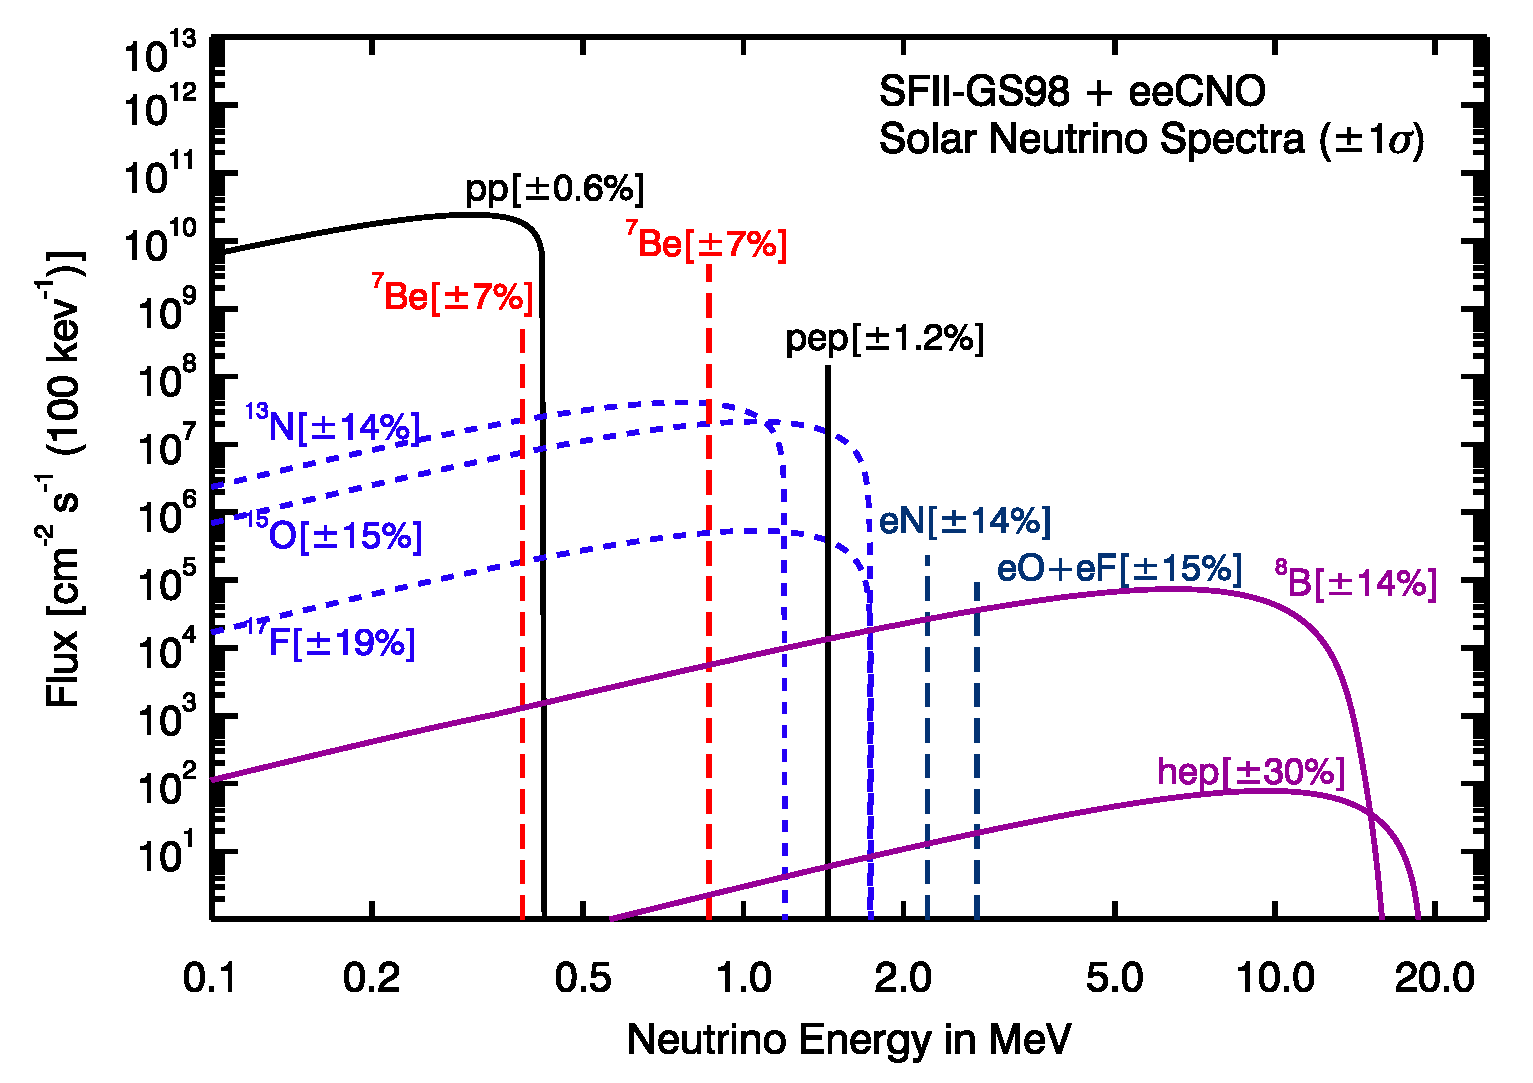
\includegraphics[width=0.85\linewidth]{theory/figure3}
    \caption[The solar neutrino flux produced by all the reactions inside Sun's core]{Solar neutrino flux produced by all the reactions inside the Sun's core. Picture taken from \cite{serenelliAliveWellShort2016}.}
    \label{fig:sun_flux}
\end{figure}

Neutrinos from the Sun come from fusion reaction chains taking place inside the Sun's core. An energy spectrum of the neutrino flux is presented in \autoref{fig:sun_flux}. The detection principle relied on the use of  the capture process $\PGne + ^{37}\mathrm{Cl} \to ^{37}\mathrm{Ar} + \Pem$, with a threshold of \SI{814}{keV}, making only $^7$Be and $^8$B flux detectable by the experiment. The produced $^{37}$Ar decayed with a half-life of $\SI{34.8}{days}$ and was measured by means of a proportional chamber. Despite the huge number of neutrinos from solar flux ${\sim}\SI{6e10}{cm^{-2}\ s^{-1}}$, only 1.7 events were expected each day \cite{bahcallStandardSolarModels1982,bahcallNewSolarOpacities2005}; however, the total flux collected by the Homestake Mine experiment amounted to an observed flux of \num{0.48(4)} neutrino interactions per day \cite{clevelandMeasurementSolarElectron1998}. 
To investigate the origin of this flux deficit, even in other components of the proton-proton ($\Pp\Pp$) and carbon–nitrogen–oxygen (CNO) processes in the Sun's core,  multiple experiments were developed, with the aim of investigating the lower part of the energy spectrum. In particular, neutrinos from the $\Pp\Pp$ chain are the most abundant, so they were targeted to clarify this problem. In order to measure this contribution, the threshold had to be lowered. The energy spectrum of the protons from the $\Pp\Pp$ chain is, as pictured in \autoref{fig:sun_flux}, lower than the minimum detectable energy of \SI{814}{\kilo\electronvolt}, achieved with previous experiments.
Using gallium, or gallium-doped targets, by means of the neutrino capture process $\PGne + ^{71}\mathrm{Ga} \to ^{71}\mathrm{Ge} + \Pem$, with a threshold energy of \SI{233}{keV} it is possible to detect neutrinos from the $\Pp\Pp$ chain. Four experiments followed this idea: the SAGE experiment at Baksan \cite{collaborationMeasurementSolarNeutrino1999}, using \SI{50}{t} of liquid metallic gallium, and the GALLEX \cite{hampelGALLEXSolarNeutrino1999} experiment at \emph{Laboratori Nazionali del Gran Sasso} (LNGS), using gallium chloride, $\mathrm{GaCl_3}$, followed by the GNO experiment; their data were used for a combined analysis \cite{hampelGALLEXSolarNeutrino1999,altmannGNOSolarNeutrino2000}. These results highlighted that also for this lower region of the energy spectrum the model was inconsistent with the data.  The same was shown by the results from the SAGE collaboration \cite{collaborationMeasurementSolarNeutrino1999}.
This set of anomalous measurements is referred to the ``solar neutrino problem''. 

The landscape evolved in 1998 with the observation of atmospheric neutrinos by the Kamiokande and Super-Kamiokande experiments. While the radiochemical detectors measure the reaction rate integrated between extractions, the real-time measurement of solar neutrinos was possible with this type of detector. The Kamiokande detector was a \SI{3000}{t} water-Cherenkov detector in the Kamioka mine. Super-Kamiokande (SK), the successor of Kamiokande, started operation in 1996. It is a large upright cylindrical water Cherenkov detector containing \SI{50}{kt} of pure water. An inner volume of \SI{32}{kt} of water was surrounded by \num{11000} photomultiplier tubes (PMT), detecting the Cherenkov radiation from the particles inside the volume. Both Kamiokande and Super-Kamiokande can detect solar neutrinos using neutrino-electron elastic scattering (ES), $\HepParticle{\PGn}{\ell}{} \Pem \to \HepParticle{\PGn}{\ell}\ {}\ \Pem$. The results of Kamiokande and SK for $\PGne$ES events still showed a decrease of the observed flux \cite{super-kamiokandecollaborationSolarNeutrinoMeasurements2016}\[
    (\mathrm{2.308\pm0.020\ (stat.)^{+0.039}_{-0.040}\ (syst.)})\times \num{e6}\ \si{cm^{-2}\ s^{-1}},
\] with respect to the expected flux of \SI{5.46+-0.66}{cm^{-2}\ s^{-1}}. %This constitutes the ``atmospheric neutrino problem''. 

% atmospheric neutrino anomaly...
The Kamioka water Cherenkov detector, as well as the Irvine-Michigan-Brookhaven (IMB) water Cherenkov detector, was also able to detect, other than electrons and electron neutrinos coming from the Sun's core, muons and muon neutrinos. These contributions are predicted to be originating in Earth's atmosphere as a result of the interaction of primary cosmic rays. Both the Kamioka and the IMB experiments observed a deficit \cite{hirataExperimentalStudyAtmospheric1988, casperMeasurementAtmosphericNeutrino1991} of neutrinos from what was expected. These anomalous measurements, among others, constitute the ``atmospheric neutrino problem'' \cite{Lipari:1996bi}. Atmospheric neutrinos come from interactions between cosmic rays and nuclei in the atmosphere, leading to the production of charged mesons, which then decay. One of the leading channels of this chain is the pion decay, $\PGppm\to\PGmpm+\brabar{\PGnGm}$, and the subsequent muon decay, $\PGmpm \to \Pepm + \brabar{\PGnGm} + \brabar{\PGne}$, implying  a flavour ratio $(\PGnGm + \PAGnGm) / (\PGne + \PAGne) = 1/2$. Both Kamiokande experiment as well as the IMB experiment measured the flavour ratio, loosely referred to as $(\PGm/\Pe)_\mathrm{obs}$, which, compared to the theory calculation $(\PGm/\Pe)_\mathrm{theory}$, yields \cite{Lipari:1996bi} \begin{equation}
    \begin{aligned}
        R = (\PGm/\Pe)_\mathrm{obs} / (\PGm/\Pe)_\mathrm{theory} & = 0.57_{-0.07}^{+0.08}\ (\text{stat.})\pm 0.07\ (\text{syst.}) && \text{(Kamioka)} \\
        R & = 0.54 \pm 0.02\ (\text{stat.})\pm 0.07\ (\text{syst.}) && \text{(IMB-3)}
    \end{aligned}
\end{equation}

The solution for this ``atmospheric neutrino problem'' came indeed from the analysis of SK atmospheric data, by following the hypothesis that neutrinos do oscillate, and hence that a deficit of muon neutrinos had to be found as an increase in the population of electron and tau neutrinos. The data collected by SK showed a good agreement for atmospheric neutrinos assuming a two-flavour oscillation \cite{ashieEvidenceOscillatorySignature2004}, with $\sin[2](2\theta) > 0.90$ and $\SI{1.9e-3}{eV^2} < \Delta m^2 < \SI{3e-3}{eV^2}$ at \SI{90}{\percent} confidence level. The confirmation of this result came from subsequent experimental efforts, especially from the OPERA experiment operating at the Laboratori Nazionali del Gran Sasso (LNGS), detecting neutrinos from the CERN Neutrinos to Gran Sasso (CNGS) beam --- the experiment  did, in fact, detect tau neutrinos \cite{collaborationDiscoveryTauNeutrino2015} from the CNGS $\PGnGm$-disappearance. 

The solution for the ``solar neutrino problem'' came in the early 2000s, with the experimental results from the Sudbury Neutrino Observatory (SNO) \cite{collaborationMeasurementRateNu_e2001}. The detector consisted of \SI{1000}{t} of heavy water, $\mathrm{D_2O}$, contained in a spherical vessel surrounded by a $\mathrm{H_2O}$ shield. An array of PMTs measured at the Cherenkov radiation produced in both $\mathrm{D_2O}$ and $\mathrm{H_2O}$. This allowed the measurements of multiple signatures of $^8$B neutrinos from the Sun's core: in addition to ES scattering in water, heavy water allowed for the detection of other interaction channels, including CC scattering off of deuterium $\PGne + \HepParticle{d}{}{} \to \Pem + \Pp+\Pp$, and NC interaction $\PGn_\ell + \HepParticle{d}{}{} \to \PGn_\ell + \Pn+\Pp$, and includes equally all neutrino flavours. Therefore, the comparison of the three fluxes (ES, CC and NC), each sensible to one or more neutrino flavours, allowed scientists to measure the full neutrino solar flux. The results of the SNO collaboration, combined with the ES events collected by SK, allowed the extraction of the full flux of neutrinos from the Sun, highlighting that flavour conversion happened also for neutrinos \cite{collaborationDirectEvidenceNeutrino2002, collaborationMeasurementRateNu_e2001, collaborationSolar8BHep2001}. The mass splitting reported by the SAGE \cite{abdurashitovMeasurementSolarNeutrino2009} and GALLEX+GNO \cite{altmannCompleteResultsFive2005} experiments was of the order of $\Delta m^2 {\sim} \SI{e-5}{eV^2}$, with the oscillation amplitude $\sin[2](2\theta)\sim0.3$. 

\begin{figure}
    \centering
    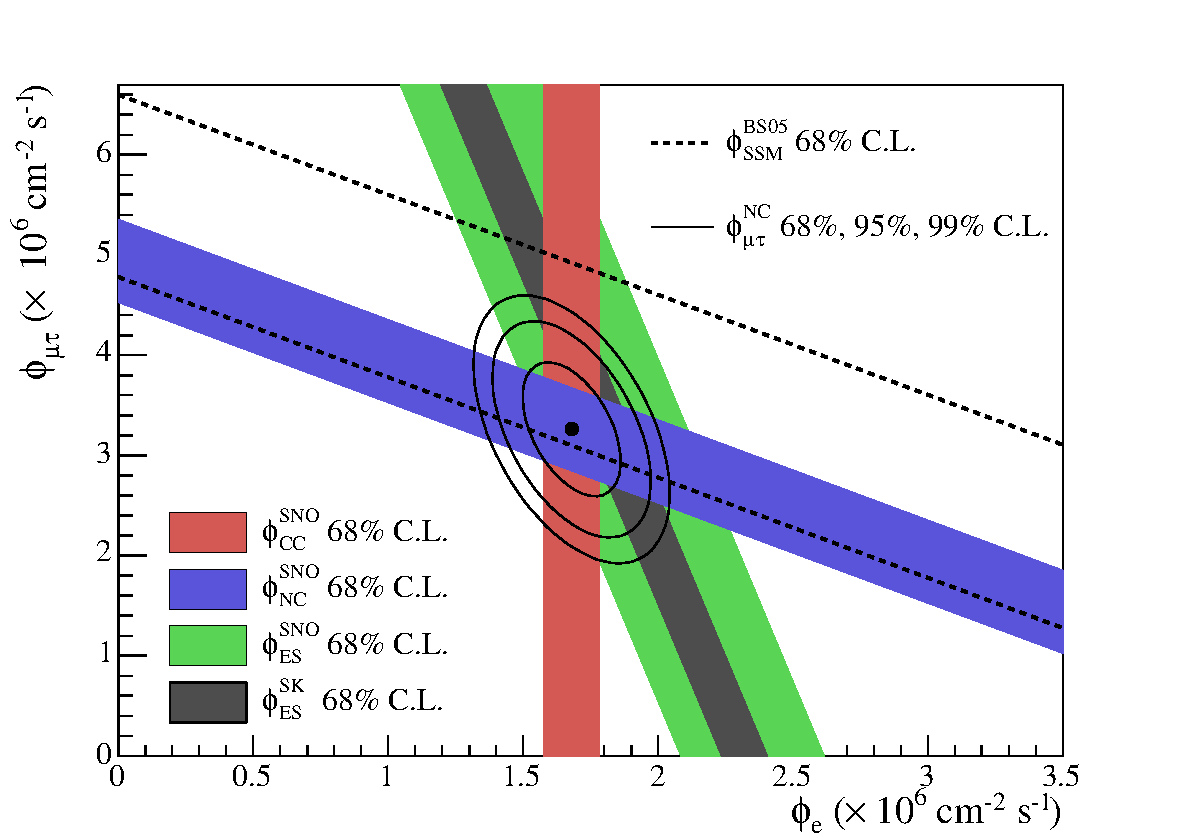
\includegraphics[width=0.85\linewidth]{theory/pnt_SNO+SK}
    \caption[SNO+SK results for the ``solar neutrino problem'']{Fluxes of $^8$B solar neutrinos, $\phi(\PGne)$, and $\phi(\HepParticle{\PGn}{\PGm,\PGt}{})$, deduced from the SNO CC, ES, and NC measurements. The standard solar model prediction \cite{bahcallStandardSolarModels1982,bahcallNewSolarOpacities2005} is also shown. The bands represent the $\pm1\sigma$ region centred around the best fit. The contours show the \SI{68}{\percent}, \SI{95}{\percent}, and \SI{99}{\percent} CL best-fit regions for the $\phi(\PGne)$ and $\phi(\HepParticle{\PGn}{\PGm,\PGt}{})$ experimental results. Figure from \cite{snocollaborationElectronEnergySpectra2005}.}
    \label{fig:sno_results}
\end{figure}


%. Theory, to formalize all
\subsubsection{Flavour oscillation formalism}

In the Standard Model of particle physics, flavour oscillation, as already mentioned, is a consequence of the fact that particles must have non-zero masses. This is the case for the hadronic sector, where flavour oscillation is regulated via the $V_\mathrm{CKM}$ matrix, which arises from the request that the mass matrix for quarks is indeed diagonal \cite{peskinIntroductionQuantumField1995}. 

In the minimal SM, neutrinos are massless, and this allows their mass eigenstates to be the same as their flavour eigenstates. Flavour eigenstates are the ones involved in interactions and determine the interaction topology that can be detected. The fact that, in the minimal SM with massless neutrinos, flavour and mass eigenstates are equivalent leads to flavour not changing as neutrinos propagate through space and time. 

As evidenced by multiple experiments in the previous sections, however, neutrinos display a very different behaviour to that predicted by the minimal SM. The observations presented before, however, do fit coherently within the framework of flavour oscillation. This framework, developed by analogy to that of flavour oscillation in the quark sector, implies that neutrinos, like quarks, must have mass. The mixing between mass and flavour eigenstates is steered by the Pontecorvo-Maki-Nakagawa-Sakata (PMNS) mixing matrix. We can define a flavour basis of eigenstates, $\PGn_\alpha = (\PGne, \PGnGm, \PGnGt)$ and a mass basis of eigenstates,  $\PGn_i = (\PGn_1, \PGn_2, \PGn_3)$. The flavour eigenstate basis of neutrinos is that which undergoes weak interaction; on the other hand, the mass eigenstate basis is that which undergoes time transformation, and the masses are their eigenvalues, dictating how each eigenstate evolves through time. We can express each base as a rotation of the other, using the complex-valued Pontecorvo-Maki-Nakagawa-Sakata (PMNS) matrix, 
\begin{equation}
    \ket{\PGn_\alpha} = \sum_{i=1}^3 U_{\mathrm{PMNS},\ \alpha i}^* \ket{\PGn_i},\quad \ket{\PGn_i} = \sum_{\alpha=1}^3 U_{\mathrm{PMNS},\ \alpha i} \ket{\PGn_\alpha}, \label{eq:basis_rotation}
\end{equation} where the Greek indices indicate the flavour eigenstate basis, and the Roman ones indicate the mass eigenstate basis.

The complex-valued $U_\mathrm{PMNS}$ matrix can be expressed as the product of three rotations and a complex phase \begin{equation}
    \begin{aligned}
        U_\mathrm{PMNS} &= \begin{pmatrix}
            1 & 0 & 0\\
            0 & \cos\theta_{23} & \sin\theta_{23} \\
            0 & -\sin\theta_{23} & \cos\theta_{23} \\
        \end{pmatrix} \times \begin{pmatrix}
            \cos\theta_{13} & 0 & \sin\theta_{13}\ e^{-i\delta} \\
            0 & 1 & 0\\
            -\sin\theta_{23}\ e^{i\delta} & 0 & \cos\theta_{23} \\
        \end{pmatrix} \times\\ 
        &\hspace{7cm}\times \begin{pmatrix}
            \cos\theta_{12} & \sin\theta_{12} & 0\\
            -\sin\theta_{12} & \cos\theta_{12} & 0\\
            0 & 0 & 1\\
        \end{pmatrix}
    \end{aligned} \label{eq:PMNS}
\end{equation} where $\theta_{ij}$ are the rotation angles, and $\delta$ is the Charge-Parity (CP) violating phase, often referred to as $\delta_\mathrm{CP}$. The theory, in the case neutrinos were Majorana particles, would require two additional phases, $\alpha_1$ and $\alpha_2$ \cite{zuberNeutrinoPhysics2020}. This is obtained by multiplying the PMNS matrix by the term \begin{equation}
    \mathrm{diag}\qty(e^{i\alpha_1/2}, e^{i\alpha_2/2}, 1).
\end{equation}

Given the rotations in \eqref{eq:basis_rotation}, neutrino oscillations arise from the time evolution of the massive eigenstates $\PGn_i$, in vacuum \cite{zuberNeutrinoPhysics2020} \begin{equation}
    \ket{\PGn_i, t} = e^{-i p \cdot x} \ket{\PGn_i, t_0 = 0} = e^{-i E\ t  + \vb p \cdot \vb x} \ket{\PGn_i, t_0 = 0}.\label{eq:time_evolution}
\end{equation}
Combining \eqref{eq:basis_rotation} and \eqref{eq:time_evolution} leads the flavour basis to oscillate as the mass eigenstates evolve in time (hereafter, $\ket{\PGn_i} = \ket{\PGn_i, t = 0}$ and the same holds for the flavour eigenstates). \begin{equation}
    \ket{\PGn_\alpha, t} = \sum_{i} U_{\alpha i}^* e^{-i E\ t  + \vb p \cdot \vb x} \ket{\PGn_i} = \sum_\beta \qty(\sum_{i} U_{\alpha i}^* e^{-i E\ t  + \vb p \cdot \vb x} U_{\beta i}) \ket{\PGn_\beta}. 
\end{equation} The probability of evolving from the initial state $\alpha$ to the final state $\beta$ at a given time $t$ is thus given by \begin{equation}
    \begin{aligned}
        P(\PGn_\alpha \to \PGn_\beta) &= \qty|\braket{\PGn_\beta}{\PGn_\alpha, t}|^2 = \qty|\sum_i\sum_j U^*_{\alpha i}U_{\beta j} \braket{\PGn_j}{\PGn_i, t}|^2 = \\
        & = \delta_{\alpha\beta} - 4\sum_{i<j} \Re[U_{\alpha i} U_{\beta i}^* U_{\alpha j}^* U_{\beta j}] \sin[2](1.26 \ \frac{\Delta m^2_{ij} }{\si{eV^2}}\ \frac{L/E}{\si{m/MeV}}) + \\
        &\qquad\qquad + 2 \sum_{i<j} \Im[U_{\alpha i} U_{\beta i}^* U_{\alpha j}^* U_{\beta j}] \sin(2\times1.26 \ \frac{\Delta m^2_{ij} }{\si{eV^2}}\ \frac{L/E}{\si{m/MeV}}). \label{eq:oscillation_nbody}
    \end{aligned}
\end{equation} under the assumptions that, for $m_i \ll p_i$, since $E_i = \sqrt{p_i^2 + m_i^2}$ in the relativistic limit, $\qty|\vb p_i|$ tends to $E_i$, and also \[
    E_ = \sqrt{p_i^2 + m_i^2} \simeq p_i + \frac{m_i^2}{2p_i} \simeq p_i + \frac{m_i^2}{2E}.
\] In Eq. \eqref{eq:oscillation_nbody} $L$ is the distance from the neutrino source to the point where neutrinos do interact (i.e. the detector), and $E$ is the neutrino energy. It is important to highlight --- especially for reasons that will be clarified in the following (see \autoref{sec:anomalies}) --- that no hypothesis about the number of neutrinos has been made to obtain such oscillation probability. Thus, equation \eqref{eq:oscillation_nbody} is valid for any number $N$ of neutrino families, as long as the mixing PMNS matrix is $N\times N$. 

Looking closely at the contributions of Eq. \eqref{eq:oscillation_nbody}, we highlight three components. The first term, $\delta_{\alpha\beta}$, correspond to the unoscillated case and is particularly important in disappearance studies. The second term, proportional to the real part of $U_{\alpha i} U_{\beta i}^* U_{\alpha j}^* U_{\beta j}$ depends on the mixing angles but is not sensible to the $\delta_\mathrm{CP}$ CP-violating complex phase. 
The CP-violation in the leptonic sector can be probed by exploiting the second term, proportional to the imaginary part. This changes sign between particles and antiparticles, so by comparing the two cases (particle and antiparticle), it is possible to measure $\delta_\mathrm{CP}$. 

Finally, some additional remarks are necessary about Eq. \eqref{eq:oscillation_nbody}. The first remark is regarding the Majorana phases, introduced briefly after Eq. \eqref{eq:PMNS}. As it is clear, if we further develop the related math of Eq. \eqref{eq:oscillation_nbody}, the $N$-flavour oscillation is not sensitive to the Majorana phases, for which a different type of search is required: this is still strictly related to the problem of neutrino masses and also to the CP violation problem \cite{brancoMajoranaNeutrinosCP1986, navasReviewParticlePhysics2024}, but not dealt with in this thesis. 

A second remark is that the oscillation probability that appears in Eq. \eqref{eq:oscillation_nbody} is valid only for neutrinos propagating through vacuum space.
In the case of propagation through matter, it is important to consider how the interaction with electrons acts on the propagation. 
This effect was first hypothesised by Mikheyev-Smirnov-Wolfenstein, hence the name MSW effect, and later confirmed by the KamLAND experiment \cite{collaborationFirstResultsKamLAND2003}. 
Briefly, starting from the hypothesis that neutrinos in matter interact coherently, the MSW effect shows how the difference between the electron neutrino flavour --- which can interact both through CC and NC coherent scatter with the nuclei ---, and the muon/tau neutrino flavours --- interacting only through NC coherent scattering --- results in a difference in their oscillation probability \cite{mikheevResonantAmplificationNeutrino1986, mikheyevResonanceAmplificationOscillations1985, wolfensteinNeutrinoOscillationsMatter1978}. 
The MSW effect and its experimental confirmations by the KamLAND experiment allow the knowledge of the sign of the mass splitting measured in solar neutrinos. 
This effect, while not relevant for short baseline experiments such as the SBN programme, is instead crucial for long baseline experiments, like the Deep Underground Neutrino Experiment \cite{kellyMatterDensityProfile2018}, and for solar neutrino experiments, which have to take into account how the oscillation probability changes as neutrinos produced in its core cross the Sun. \autoref{fig:MSW_solar_borex} shows the effects of matter oscillations for solar neutrinos, comparing the vacuum-oscillation model with the MSW effect, which does fit better wih the data. 

\begin{figure}
    \centering
    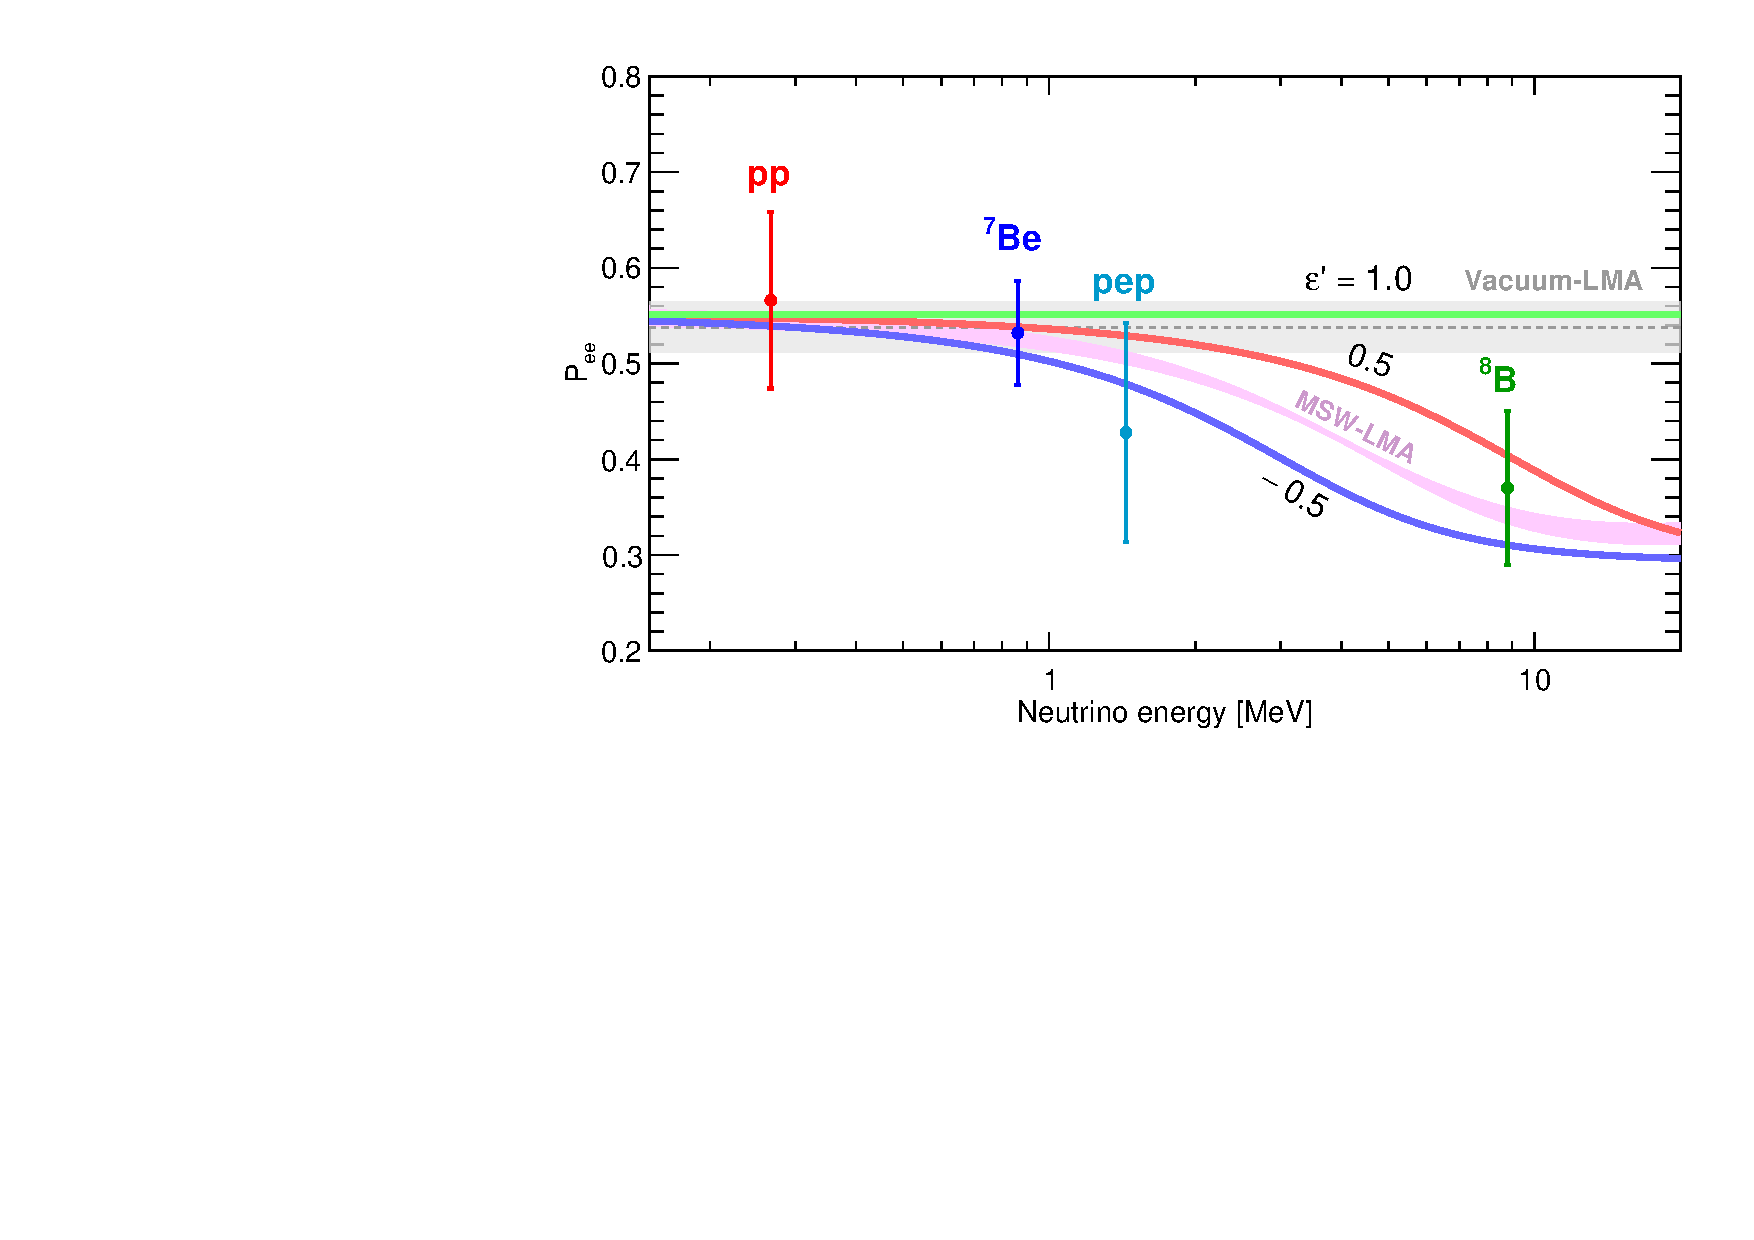
\includegraphics[width=0.85\linewidth]{theory/Pee.pdf}
    \caption[MSW effect is solar neutrinos]{Effect of the MSW matter effect on solar neutrino oscillations, comparing the data with the vacuum-oscillated model and the MSW model. Picture taken from \cite{Borexino:2019mhy}. }
    \label{fig:MSW_solar_borex}
\end{figure}

The final remark is about the experimental values of the mass splitting. With the current status of neutrino oscillation experiments, we have identified the absolute value of two mass splitting terms: one coming from the best fit of atmospheric neutrino oscillations ($\PGnGm\leftrightarrow\PGnGt$ oscillations), which is regarded as $\qty|\Delta m^2_\mathrm{Atmospheric}|$, and the other from the best fit of solar neutrino oscillations (mainly $\PGne\leftrightarrow\PGnGm$ oscillations), which is known as $\Delta m^2_\mathrm{Solar}$. The peculiarity is that these values show two orders of magnitude of difference, i.e. \begin{equation}
    \qty|\Delta m^2_\mathrm{Atmospheric}| \simeq \SI{e-3}{eV^2} \gg \Delta m^2_\mathrm{Solar} \simeq \SI{e-5}{eV^2}.\label{eq:masses_values}
\end{equation} Since we cannot know, for the atmospheric oscillations, the sign of the mass splitting, there are two possible scenarios. The first, called normal ordering or normal hierarchy (NO/NH), assumes a positive sign for both, and so $m_1 < m_2 < m_3$. The alternative assumes a negative sign for the atmospheric mass splitting, and thus $m_3 < m_1 < m_2$. \autoref{fig:ordering} shows an illustration of both NO (left) and IO (right). 
This great difference between the two mass splitting values, shown in Eq. \eqref{eq:masses_values}, can be exploited to simpplify the experimental observations. By choosing accordingly both the neutrino energy and the baseline at which neutrinos are detected from their sources, many experiments can simplify the oscillation description and assume a two-neutrino oscillation framework.

\begin{figure}
    \centering
    \begin{tikzpicture}[
        nue/.style={fill=Red!70!white},
        numu/.style={fill=ForestGreen!65!white},
        nutau/.style={fill=MidnightBlue!65!white},
        scale=0.75
    ]

        %%%%%%%%%%%%%%%%%%%%%%%%%%%%%%%%%%%%%%%%%%%%%%%%%%%%%%%%%%%%%%%%%%%%%%%%%%%%%%%%
        %%%%%% NORMAL MASS ORDERING %%%%%%%%%%%%%%%%%%%%%%%%%%%%%%%%%%%%%%%%%%%%%%%%%%%%
        %%%%%%%%%%%%%%%%%%%%%%%%%%%%%%%%%%%%%%%%%%%%%%%%%%%%%%%%%%%%%%%%%%%%%%%%%%%%%%%%

        \node[text centered] at (-3,0) {Normal ordering};
        \node[text centered] at (-0.5,0) {$\delta_\mathrm{CP}$};

        \node[text centered] at (-5.5, -.75)  {$\PGn_3$};
        \node[text centered] at (-5.5, -3.75) {$\PGn_2$};
        \node[text centered] at (-5.5, -4.75) {$\PGn_1$};

        \fill[nue] (-5,-.5) -- (-4.75,-.5) -- (-4.75,-1) -- (-5,-1) -- cycle;
        \fill[numu] (-4.75,-.5) -- (-3.,-.5) -- (-3.,-1) -- (-4.75,-1) -- cycle;
        \fill[nutau] (-3.,-.5) -- (-1,-.5) -- (-1,-1) -- (-3.,-1) -- cycle;

        \draw[black] (-5,-.5) rectangle (-1,-1);

        \node[text centered] at (-.65, -.5) {\small$\pi$};
        \node[text centered] at (-.65, -1) {\small 0};

        \fill[nue] (-5,-3.5) -- (-4.,-3.5) -- (-4.,-4) -- (-5,-4) -- cycle;
        \fill[numu] (-4.,-3.5) -- (-2.15,-3.5) -- (-3,-4) -- (-4,-4) -- cycle;
        \fill[nutau] (-2.15,-3.5) -- (-1,-3.5) -- (-1,-4) -- (-3.,-4) -- cycle;

        \draw[black] (-5,-3.5) rectangle (-1,-4);

        \node[text centered] at (-.65, -3.5) {\small$\pi$};
        \node[text centered] at (-.65, -4) {\small 0};

        \fill[nue] (-5,-4.5) -- (-2.575,-4.5) -- (-2.575,-5) -- (-5,-5) -- cycle;
        \fill[numu] (-2.575,-4.5) -- (-2.2,-4.5) -- (-1.25,-5) -- (-2.575,-5) -- cycle;
        \fill[nutau] (-2.2,-4.5) -- (-1,-4.5) -- (-1,-5) -- (-1.25,-5) -- cycle;

        \draw[black] (-5,-4.5) rectangle (-1,-5);

        \node[text centered] at (-.65, -4.5) {\small$\pi$};
        \node[text centered] at (-.65, -5) {\small 0};

        \draw[gray, line width=1mm] (-6.25, -4.85) -- (-6.25, -3.65);
        \draw[gray, line width=1mm] (-6, -.65) -- (-6, -3.85);

        \node[] at (-7.65, -4.25) {
            \begin{minipage}{1.75cm}
                \raggedleft
                Solar\\
                $\sim \SI{e-5}{eV^2}$
            \end{minipage}
        };

        \node[] at (-3.85, -2.25) {
            \begin{minipage}{2.55cm}
                Atmospheric\\
                $\sim \SI{e-3}{eV^2}$
            \end{minipage}
        };

        %%%%%%%%%%%%%%%%%%%%%%%%%%%%%%%%%%%%%%%%%%%%%%%%%%%%%%%%%%%%%%%%%%%%%%%%%%%%%%%%
        %%%%%% INVERTED MASS ORDERING %%%%%%%%%%%%%%%%%%%%%%%%%%%%%%%%%%%%%%%%%%%%%%%%%%
        %%%%%%%%%%%%%%%%%%%%%%%%%%%%%%%%%%%%%%%%%%%%%%%%%%%%%%%%%%%%%%%%%%%%%%%%%%%%%%%%

        \node[text centered] at (+3,0) {Inverted ordering};
        \node[text centered] at (+5.5,0) {$\delta_\mathrm{CP}$};

        \node[text centered] at (0.5, -.75)  {$\PGn_2$};
        \node[text centered] at (0.5, -1.75) {$\PGn_1$};
        \node[text centered] at (0.5, -4.75) {$\PGn_3$};

        \fill[nue] (1,-.5) -- (2.,-.5) -- (2.,-1) -- (1,-1) -- cycle;
        \fill[numu] (2.,-.5) -- (3.85,-.5) -- (3,-1) -- (2,-1) -- cycle;
        \fill[nutau] (3.85,-.5) -- (5,-.5) -- (5,-1) -- (3.,-1) -- cycle;

        \draw[black] (1,-.5) rectangle (5,-1);

        \node[text centered] at (5.35, -.5) {\small$\pi$};
        \node[text centered] at (5.35, -1) {\small 0};

        \fill[nue] (1,-1.5) -- (3.425,-1.5) -- (3.425,-2) -- (1,-2) -- cycle;
        \fill[numu] (3.425,-1.5) -- (3.8,-1.5) -- (4.75,-2) -- (3.425,-2) -- cycle;
        \fill[nutau] (3.8,-1.5) -- (5,-1.5) -- (5,-2) -- (4.75,-2) -- cycle;

        \draw[black] (1,-1.5) rectangle (5,-2);

        \node[text centered] at (5.35, -1.5) {\small$\pi$};
        \node[text centered] at (5.35, -2) {\small 0};

        \fill[nue] (1,-4.5) -- (1.25,-4.5) -- (1.25,-5) -- (1,-5) -- cycle;
        \fill[numu] (1.25,-4.5) -- (3.,-4.5) -- (3.,-5) -- (1.25,-5) -- cycle;
        \fill[nutau] (3,-4.5) -- (5,-4.5) -- (5,-5) -- (3.,-5) -- cycle;

        \draw[black] (1,-4.5) rectangle (5,-5);

        \node[text centered] at (5.35, -4.5) {\small$\pi$};
        \node[text centered] at (5.35, -5) {\small 0};

        \draw[-*, Red!65!black, shorten >=-2pt] (-4, -5.5) node[below, text centered] {$\PGne$} -- (-4, -5);
        \draw[-*, ForestGreen!65!black, shorten >=-2pt] (-2, -5.5) node[below, text centered] {$\PGnGm$} -- (-2, -5);
        \draw[-*, MidnightBlue!65!black, shorten >=-2pt] (-1.15, -5.5) node[below, text centered] {$\PGnGt$} -- (-1.15, -5);

        \draw[gray, line width=1mm] (6.1, -4.85) -- (6.1, -1.65);
        \draw[gray, line width=1mm] (5.85, -.65) -- (5.85, -1.85);

        \node[] at (7.25, -.85) {
            \begin{minipage}{1.75cm}
                Solar\\
                $\sim \SI{e-5}{eV^2}$
            \end{minipage}
        };

        \node[] at (3.85, -3.25) {
            \begin{minipage}{2.55cm}
                \raggedleft
                Atmospheric\\
                $\sim \SI{e-3}{eV^2}$
            \end{minipage}
        };

        \draw[-Latex, very thick] (-7.25, -2.) node[below] {$m_\PGn^2$} -- (-7.25, -0.5);
        
    \end{tikzpicture}
    \caption[Neutrino mass ordering]{The two scenarios for neutrino mass ordering:  the normal ordering (NO), on the left, and the inverted ordering (IO), on the right. The shaded area represents the mixing angles, or the fraction of each flavour contained in the mass eigenstates. Additionally, the dependence on the CP-violating phase effect is shown, with its value ranging from 0 to $\pi$. Figure adapted from \cite{menaUnifiedGraphicalSummary2004}.}
    \label{fig:ordering}
\end{figure}

%. Presenta status
\subsubsection{Present status}

In order to assess the entity of neutrino oscillations, we need to measure the parameters of the PMNS matrix. 
As we can read from Eq. \eqref{eq:PMNS}, it depends on three angles and a complex phase, so, in order to measure it correctly, multiple experimental measurements must be carried out. 
Additionally, one aims at knowing the precise value of the mass splittings. 
Each parameter can be accessed by exploiting different neutrino sources in order to vary the baseline and the energy or the $L/E$ ratio of the measured interaction to pinpoint each parameter in the phase space. 
Additionally, oscillation measurements are classified either as ``appearance'' experiments, where the oscillation from a given flavour $\alpha$ to another $\beta$ is measured, or as ``disappearance'' measurements, where the probability $P(\PGn_\alpha \to \PGn_\alpha) = 1 - \sum_{\beta\neq\alpha} P(\PGn_\alpha \to \PGn_\beta)$ of getting the same flavour at different distances from the sources is tested. 

The distance of the detector from the experimental source is usually selected to maximise the sensitivity to a precise mass splitting, $\Delta m^2 {\sim} E/L$. 

Recently, the precision with which these parameters are determined reached a percent value, allowing neutrino oscillation physics to move from the ``discovery'' to the ``precision'' era. 

\paragraph{Solar neutrino observations} Solar neutrinos were the first probe for neutrino oscillations and still are an interesting source with multiple search channels for both neutrino oscillations as well as precise measurements of the multiple components of the solar neutrino energy flux, shown in \autoref{fig:sun_flux}, down to a precision ranging from \qtyrange{2}{15}{\percent} in all major channels (pp, CNO, $^7$Be) \cite{BOREXINO:2020hox, Kumaran:2021lvv}, with the only exception of the hep $\mathrm{^3He} + \Pp \to \mathrm{^4He} + \Pep + \PGne$ process, which is expected to be studied by the JUNO detector with increased sensitivity \cite{JUNO:2023zty}. Given that the energy range  for solar neutrinos is $\SI{233}{keV} \leq E_\PGn \lesssim \si{MeV}$, and the baseline $L$ corresponding to the distance between the Sun and Earth, the $E/L$ ratio allows the measurement of $\Delta m^2_\mathrm{Solar} {\sim} \SI{e-5}{eV^2}$. This implies that the measured neutrino flux can be described assuming a two-state mixing scheme and thus $\sin^22\theta_{12}$ can be measured. Precise measurements are the result of multiple years of observations from multiple detectors, leading to an allowed region at $3\sigma$ for the oscillation parameters $\Delta m_{21}^2$ from \qtyrange{6.92e-5}{8.05e-5}{eV^2} and $\sin^2\theta_{12}$ from \numrange{0.275}{0.345}. These results are the combination of measurements from the Soviet-American Gallium Experiment (SAGE) \cite{abdurashitovMeasurementSolarNeutrino2009}, the GALLium EXperiment (GALLEX), the Gallium Neutrino Observatory (GNO) \cite{altmannCompleteResultsFive2005}, the Kamiokande and SK experiments \cite{collaborationSolarNeutrinoMeasurements2024}, the BOREXINO experiment \cite{agostiniExperimentalEvidenceNeutrinos2020} and the Kamioka Liquid scintillator ANtineutrino Detector (KamLAND) experiment \cite{kamlandcollaboration$^7mathrmBe$SolarNeutrino2015}. 

\paragraph{Atmospheric neutrinos} The $L/E$ ratio for neutrinos, with an energy spectrum from \SI{0.1}{GeV} to \SI{10}{TeV}, and detected at baselines compatible with the thikness of the atmosphere from \qtyrange{15}{12700}{\km}, generated mostly by pion decays in the atmosphere allows exploring the $\PGnGm\leftrightarrow\PGnGt$ oscillation phase space that is characterised by a mass splitting $|\Delta m_{32}^2| = |\Delta m_\mathrm{Atmospheric}^2| {\sim} \SI{e-3}{eV^2}$, and so allows for the determination of $\sin\theta_{23}$. Atmospheric neutrino oscillations have been studied by the Kamiokande experiment \cite{hirataExperimentalStudyAtmospheric1988} and its successor, Super-Kamiokande \cite{ashieEvidenceOscillatorySignature2004}, by the MACRO experiment \cite{collaborationMatterEffectsUpwardGoing2001}, and also by neutrino telescopes, such as the ANTARES experiment and the IceCube experiment. Novel experiments will join this research, such as the KM3NeT-ORCA telescope, the successor of the ANTARES experiment, the Hyper-Kamiokande experiment, the JUNO experiment, and the DUNE experiment. 

\paragraph{Accelerator neutrinos} A phase space similar to that of atmospheric neutrino oscillations can be explored by the accelerator neutrino experiments, especially at long baselines. Conventional neutrino beams from accelerators are produced by colliding high-energy particles onto a target --- usually $\Pp$ on a $^7$Be target --- thereby producing $\PGp$ and $\PK$, which then decay into neutrinos. The branching ratio of $\PGpp \to \PGmp\PGnGm$ is ${\sim}\SI{100}{\percent}$, and a minimal beam contamination from $\PGne/\PAGne$ (less then \SI{0.5}{\percent} in the Booster Neutrino Beam operatin at Fermilab, and similar $<\SI{1}{\percent}$ was also obtained by the CNGS beam) comes from kaon decays. The values of neutrino energy and baseline are chosen to maximise the oscillation probability, either for studying the atmospheric mass splitting $\qty|\Delta m_{21}^2| \simeq \SI{2.5e-3}{eV^2}$, with the first oscillation maximum at $L/E \simeq \SI{500}{GeV/km}$, or for testing the $\Delta m^2 {\sim} \SI{1}{eV^2}$ splitting at ${\sim} \SI{1}{km}$ baselines. 

The present landscape of the accelerator neutrino experiments is vast, from the first experiments being the K2K and MINOS experiments --- exploring the values of $\Delta m_{31}^2$ and $\Delta m_{32}^2$, by studying the $\PGnGm$-disappearance channel --- to their successors, the T2K experiment, building upon the K2K experiment, employing Super-Kamiokande as its far detector at \SI{295}{km}, and the NOvA experiment, collecting neutrinos from the Neutrino at the Main Injector (NuMI) beam at a baseline of \SI{810}{km}. Both T2K and NOvA measured $\Delta m_{31}^2$, $\Delta m_{32}^2$ , and $\sin\theta_{23}$ by measuring both the $\PGne$-appearance and $\PGnGm$-disappearance channels from a pure $\PGnGm$ beam \cite{abeObservationElectronNeutrino2014, collaborationMeasurementsNeutrinoOscillation2023, collaborationConstraintsOscillationParameters2017}. Additionally, both experiments performed a measurement of the $\delta_\mathrm{CP}$ violating phase of the PMNS matrix. The T2K experimental results showed a preference towards $\delta_\mathrm{CP}{\sim}\pi/2$ \cite{collaborationMeasurementsNeutrinoOscillation2023}, whereas the NOvA data showed a preference towards $\delta_\mathrm{CP}\sim3\pi/2$ \cite{collaborationConstraintsOscillationParameters2017}. 

\paragraph{Reactor antineutrinos} Nuclear fission reactors give a substantial flux of electron antineutrinos in the \si{MeV} region, through $\beta$-decay of radioactive isotopes created during the fission process, primarily $^{235}$U, $^{238}$U, $^{239}$Pu, and $^{241}$Pu; $\PAGne$ are then detected at different baselines${\sim}\SI{1}{km}$. Charged current events cannot happen, given the available phase space, for $\PAGnGm$ or $\PAGnGt$ since they require more energy to produce $\PGm$ or $\PGt$ in the final state than what is accessible, so flavour oscillation for such experiments is only accessible through the $\PAGne$-disappearance channel. The detection mechanism relies on the inverse beta decay $\Pp + \PAGne \to \Pep + \Pn$, where the signal from the prompt $\Pep$ and the delayed $\PGg$ (with the energy depending on the type of scintillator; \SI{2.2}{MeV} for hydrogen, \SI{8}{MeV} when it is loaded with gallium) from the thermalisation of the neutron helps separate it from the background. 

The Kamioka Liquid scintillator ANtineutrino Detector (KamLAND) experiment was a pioneer experiment, measured neutrinos from multiple nuclear reactors at ${\sim} \SI{180}{km}$ from the source, observing a ratio of inverse $\beta$ decay over the predicted flux of \begin{equation}
    \mathrm{0.611 \pm 0.085\ (stat.) \pm 0.041\ (syst.)},
\end{equation} showing evidence for $\PAGne$-disappearance at \SI{99.95}{\percent} confidence level \cite{collaborationFirstResultsKamLAND2003}. 

Reactor antineutrino experiments also showed very high sensitivity to the $\theta_{13}$ mixing angle. This is possible in the case of a short baseline ${\sim} \SI{1}{km}$, as in the case of the Double Chooz experiment \cite{abeIndicationDisappearanceReactor2012}, the Daya Bay experiment \cite{anObservationElectronantineutrinoDisappearance2012}, and the RENO experiment \cite{kimObservationReactorElectron2012}, which found, respectively, \begin{align}
    &\begin{aligned}
        \sin^22\theta_{13} &= \mathrm{0.086 \pm 0.041\ (stat.) \pm 0.030\ (syst.)},\\
        & \text{or}\ 0.017 < \sin^22\theta_{13} < 0.16\ \text{at \SI{90}{\percent} CL}
    \end{aligned} && \text{(Double Chooz)}\\
    &\sin^22\theta_{13} = \mathrm{0.092 \pm 0.016\ (stat.) \pm 0.005\ (syst.)} && \text{(Daya Bay)}\\
    &\sin^22\theta_{13} = \mathrm{0.113 \pm 0.013\ (stat.) \pm 0.019\ (syst.)} && \text{(RENO)}
\end{align} 

\section{Short baseline anomalies}\label{sec:anomalies}

It is clear at this point that the three-state mixing scheme of neutrino flavour oscillation is well established, from the empirical point of view, leading to the clear necessity of a ``minimal'' extension of the standard model in order to introduce neutrino masses. Since the mass and size of neutrinos is very different from other particles of the standard model, generating their masses would require a novel mechanism. Multiple beyond SM physics (BSM) models have been developed \cite{navasReviewParticlePhysics2024, Arguelles:2019xgp}, all requiring the addition of particle content to the SM; however, in spite of the well established evidence for neutrino masses, no direct measurement has been made to date, and no model is currently preferred over the others \cite{navasReviewParticlePhysics2024}. 

In addition to these open questions, in the past twenty years the picture has been complicated by some anomalous observations. Multiple short-baseline experiments, operating at a baseline $L$ with neutrino energy $E$ such that $L/E {\sim} \mathcal O (\SI{10}{m}/\si{MeV})$, observed either a deficit or an excess of events of neutrino interactions in multiple channels and with different neutrino sources \cite{aceroWhitePaperLight2024}. The combination of these anomalies at short baselines of ${\sim}\SI{1}{km}$ hints at the existence of a fourth neutrino flavour with a mass splitting $\Delta m^2 {\sim} \SI{1}{eV}$. This, combined with the fact that only three ``active'' (i.e. interacting) families of neutrinos are compatible with all the experimental results so far \cite{decampPreciseDeterminationNumber1990}, lead to the ``sterile'' neutrino hypothesis, i.e. a neutrino singlet in the SM that does not undergo weak interaction and is subject only to gravitational force. Here a more detailed picture of the different short baseline anomalies recorded is presented. 


% that could be hinting at the possibility of a fourth neutrino state. This was suggested by a series of short-baseline experiments --- for which $L/E {\sim} \mathcal O (\SI{10}{m}/\si{MeV})$ }. 

\begin{figure}
    \centering
    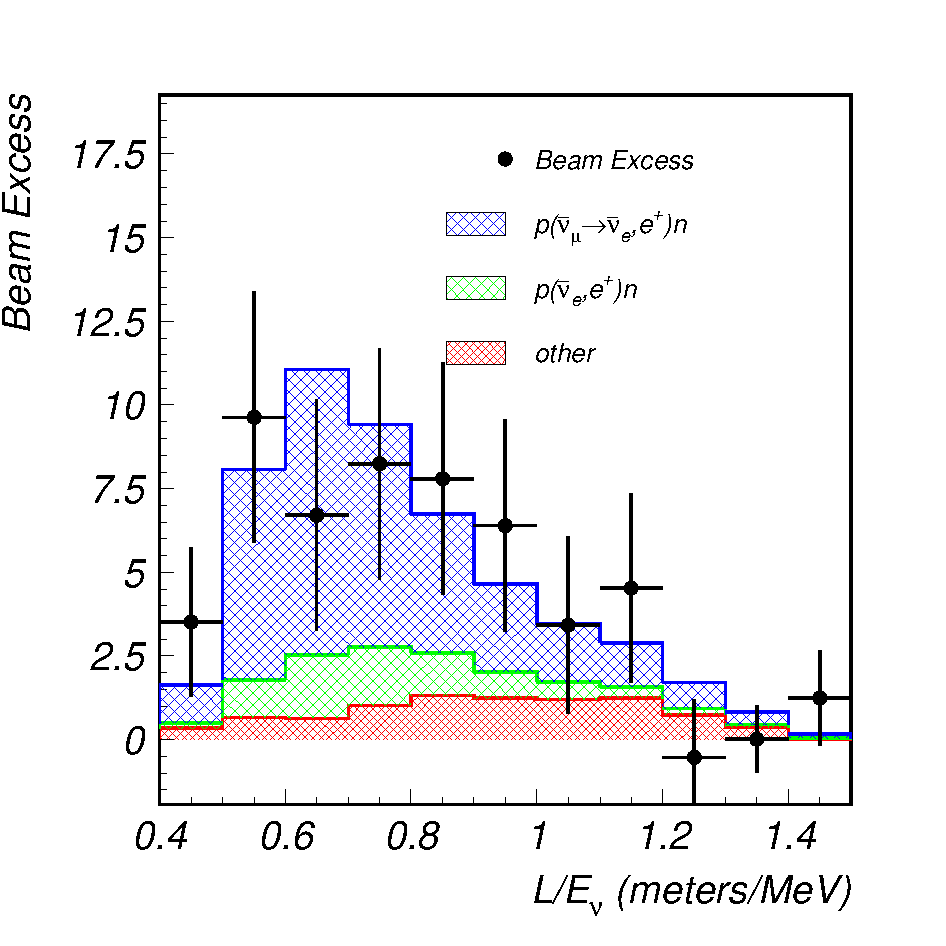
\includegraphics[width=0.65\linewidth]{anomalies/Fig24_elec_loe_rcut.pdf}
    \caption[LSND anomalous excess]{LSND anomalous events as a function of $L/E_\PGn$ for a subset of total events. The red and green shaded areas account for the the different parts of the beam flux, whereas the back dots show the overlayed data. The blue area shows the best fit under the hypothesis of a sterile-state mediated oscillation. More information can be found in Ref. \cite{aguilarEvidenceNeutrinoOscillations2001}, from which the figure was taken.}
    \label{fig:LSND_excess}
\end{figure}

% The Liquid Scintillator Neutrino Detector (LSND) at Los Alamos Laboratories measured $\PAGne$ produced by the oscillation of a $\PAGnGm$ beam using a liquid scintillator and observed an excess (shown in \autoref{fig:LSND_excess}) of electron antineutrinos, with a $3.8\sigma$ tension from the three-flavour mixing scenario \cite{aguilarEvidenceNeutrinoOscillations2001}. This result was later tested by the MiniBooNE experiment with a different neutrino source and at a different baseline. The MiniBooNE collaboration reported an analogous signal of excess of $\PGne$ in a $\PGnGm$ beam with a significance of $4.8\sigma$ \cite{collaborationCombined$n_mtoN_e$2012}. Reactor antineutrino measurements, which played a significant role in establishing the three-flavour oscillation paradigm for neutrinos, also observed a decrease in flux of electron antineutrinos at baseline distances $<\SI{100}{m}$, with a ratio to the prediction $R=\num{0.976+-0.024}$ \cite{mentionReactorAntineutrinoAnomaly2011} --- effect known as ``reactor antineutrino anomaly''. Furthermore, GALLEX and SAGE \cite{collaborationMeasurementSolarNeutrino1999, hampelGALLEXSolarNeutrino1999} employed radiochemical techniques to detect solar neutrinos with gallium detectors; calibration was performed in both cases using megacurie radioactive sources, either $^{51}$Cr or $^{37}$Ar, and returned anomalous fluxes in the $\PGne$-disappearance channel, with an observed-to-expected ratio $R=\num{0.86\pm0.05}$, showing a $2.2\sigma$ statistical significance. This result was later corroborated by the measurements from the BEST experiment: combining all radiochemical measurements increased significance of the so called ``Gallium Anomaly'' (GA) to $\sim4\sigma$ \cite{elliottGalliumAnomaly2023}. 

\paragraph{Pion decay-at-rest accelerator experiments} Pion decay-at-rest generate a very pure muon antineutrino flux with a mean energy of $E_\PAGn\simeq \SI{30}{MeV}$. As such, a detector placed at a relatively short baseline ${\sim}\SI{30}{m}$ from the source is sensitive to oscillation with a mass splitting ${\sim}\SI{1}{eV^2}$. Two major experiments employed this technology to produce neutrino beams, the LSND (Liquid Scintillator Neutrino Detector) and the KARMEN (KArlsruhe Rutherford Medium Energy Neutrino) experiments. Of the two, LSND had the highest sensitivity and observed the ``LNSD anomaly''. The KARMEN experiment saw no evidence of such an anomaly, and it is thus considered a ``null'' experiment for the sterile neutrino framework \cite{collaborationUpperLimitsNeutrino2002}. 

The LSND experiment at Los Alamos Laboratories measured $\PAGne$ produced by the oscillation of a $\PAGnGm$ beam using a liquid scintillator and observed an excess (shown in \autoref{fig:LSND_excess}) of electron antineutrinos, with a $3.8\sigma$ tension from the three-flavour mixing scenario \cite{aguilarEvidenceNeutrinoOscillations2001}. The LSND experiment consisted of a cylindrical tank of \SI{8.3}{m} of height and a diameter of \SI{5.7}{m}, placed horizontally, filled with \SI{167}{metric\ tons} of mineral oil. LNSD detected electron antineutrinos from a beam of muon antineutrinos, produced by pions decaying at rest (DAR). The pions were produced by protons with $E_\Pp\simeq \SI{798}{MeV}$ hitting a water target that produced stopped pions. The signal selection relied on the measurement of both the scintillation light and the Cherenkov light cone produced by the positron (see figure \ref{fig:LSND_detector} for a schematic illustration) correlated with a delayed \SI{2.2}{MeV} photon signal produced by neutron capture. Scintillation and Cherenkov light were collected by means of 1220 PMTs. The LNSD data showed an excess of events of $\mathrm{87.9 \pm 22.4\ (stat.) \pm 6.0\ (syst.)}$, compatible with the hypothesis of a two-flavour oscillation $\PAGnGm\to\PAGne$. The fit pointed toward an oscillation amplitude of $\sin^22\theta_{\PGm\Pe} \simeq \num{0.003}$ and a mass splitting of $\Delta m^2 \simeq \SI{1.2}{eV^2}$, resulting in the allowed regions at \SI{90}{\percent} CL and \SI{99}{\percent} CL shown in figure \ref{fig:LSND_lhd} \cite{aguilarEvidenceNeutrinoOscillations2001}. 

\begin{figure}
    \centering
    \subfloat[]{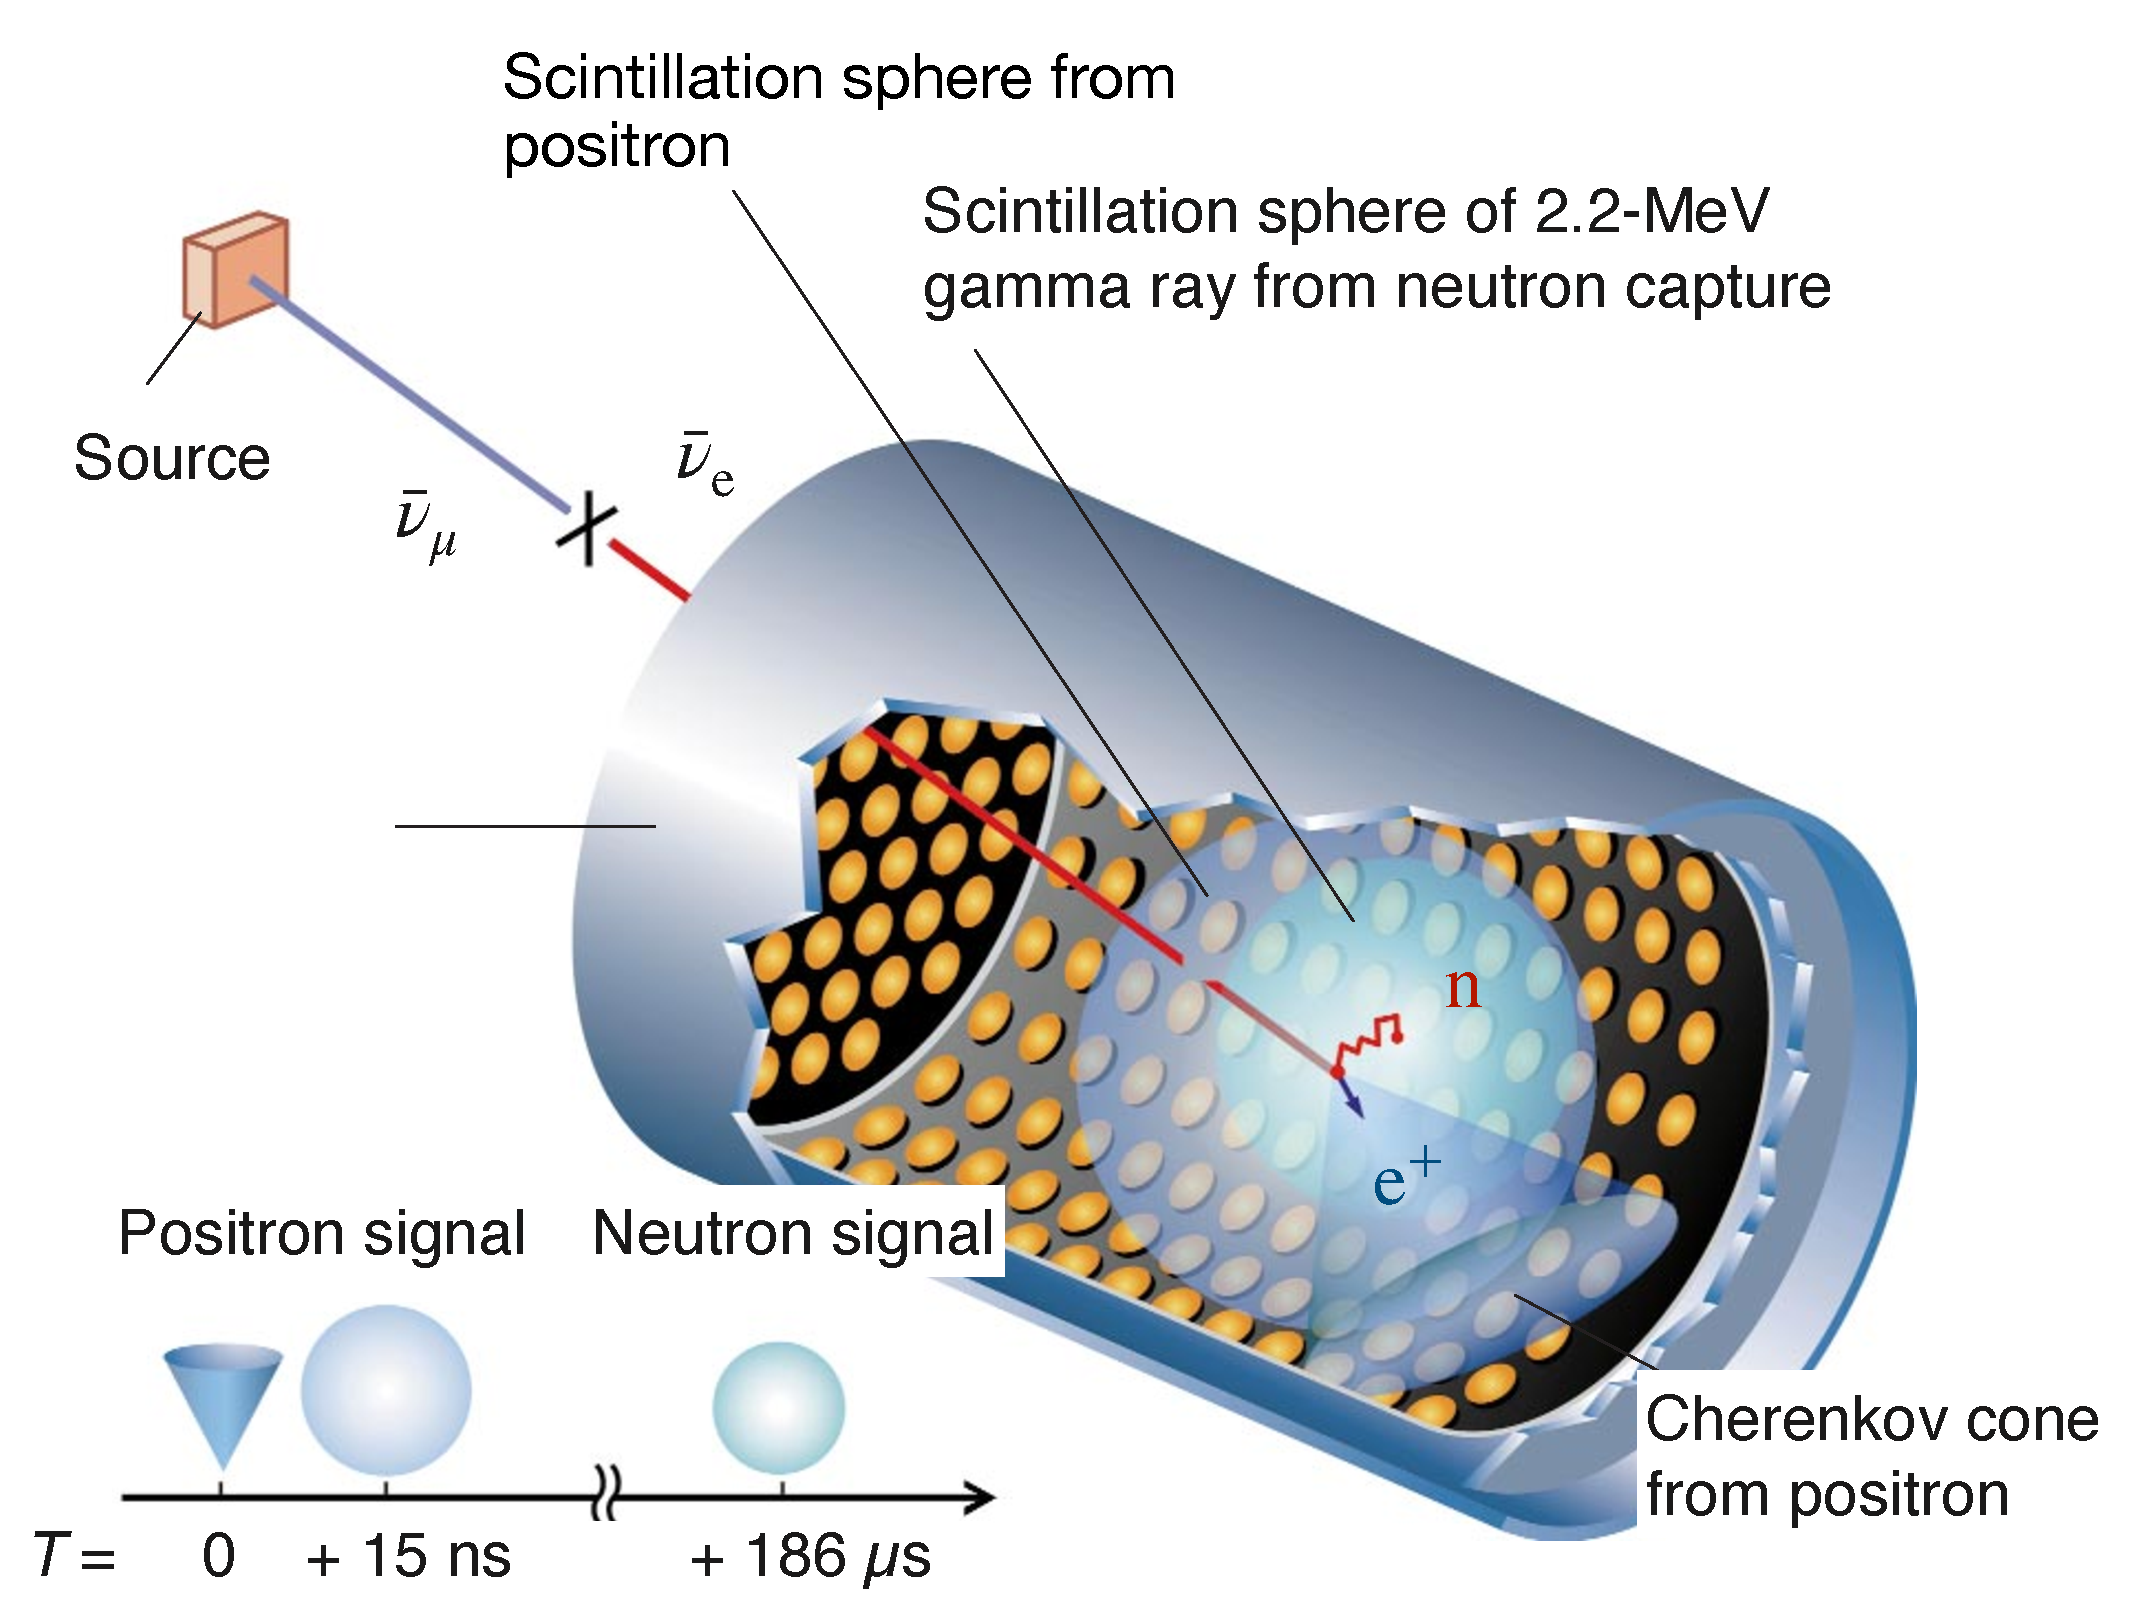
\includegraphics[width=0.5\linewidth, trim={0 -4cm 0 0}]{anomalies/LNSD.pdf}\label{fig:LSND_detector}}
    \subfloat[]{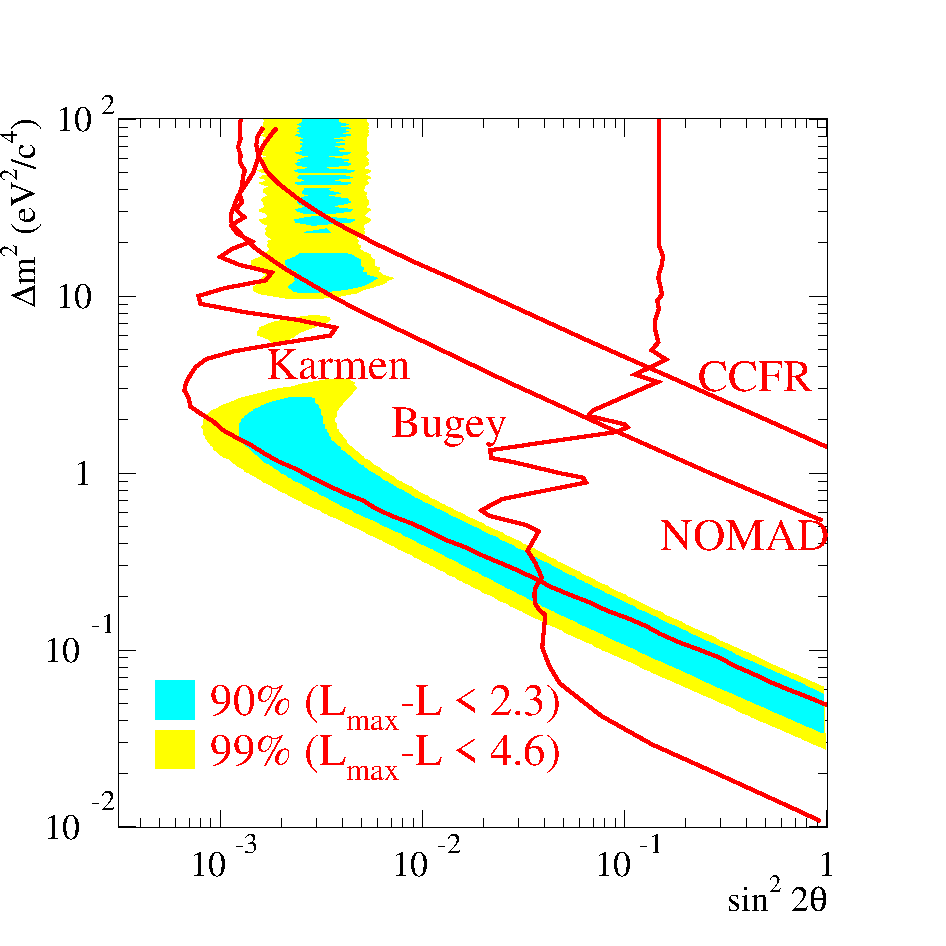
\includegraphics[width=0.5\linewidth]{anomalies/Fig27_lhd.pdf}\label{fig:LSND_lhd}}
    \caption[The LNSD detector and results]{\ref{sub@fig:LSND_detector} Illustration of the LNSD detector at the Los Alamos Laboratories. In the illustration a typical electron antineutrino interaction is displayed, with both the prompt scintillation light and Cherenkov cone from the positron, as well as the light emitted by the subsequent neutron capture. Figure adapted from \cite{louisThousandEyesStory1997}. \ref{sub@fig:LSND_lhd} Allowed regions from the LNSD fit to the sterile neutrino hypothesis in the oscillation parameter phase space. Figure taken from \cite{aguilarEvidenceNeutrinoOscillations2001}}
    \label{fig:LSND}
\end{figure}

\paragraph{Pion decay-in-flight accelerator experiments} LNSD's evidence for this oscillation prompted subsequent searches. This is why pion decay-in-flight (DIF) was selected as a valid production mechanism: it produces a pure $\brabar{\PGnGm}$ beam with higher energy, providing the opportunity for an independent test at a higher baseline. This was accomplished using the Booster Neutrino Beam (BNB), providing a \SI{99.5}{\percent} pure muon neutrino beam with a mean energy of ${\sim} \SI{700}{MeV}$, in conjunction with the MiniBooNE Cherenkov detector at the Fermi National Accelerator Laboratories (Fermilab) in Illinois. The design of this experiment was adjusted to allow the phase space to align with that of the LNSD experiment: $E/L {\sim} \SI{30}{MeV}/\SI{30}{m}$ for the LNSD experiment, so the same was accomplished by placing the MiniBooNE detector at \SI{540}{m}. The MiniBooNE detector consisted of a single tank containing \SI{818}{\tonne} of mineral oil. The detection technique was based on the measurement of Cherenkov radiation that was possible thanks to 1520 PMTs located inside the detector tank. The Cherenkov light cone was used to separate between $\PGne$CC and $\PGnGm$CC events; the purity of the present selection was undermined by the presence of backgrounds coming mainly from NC interactions inside the tank and NC $\PGpz$ interactions where one photon from the $\PGpz$ decay is lost. The MiniBooNE experiment took data from 2002 to 2019, collecting a total of \SI{18.75e20}{POT} (protons-on-target) interactions with both a neutrino mode and an antineutrino mode, showing an excess of events in the signal region $\SI{200}{MeV} < E_\PGn^\mathrm{QE} < \SI{475}{MeV}$, with a statistical significance of $4.8\sigma$ \cite{collaborationUpdatedMiniBooNENeutrino2021}. This excess is known by the name of Low Energy Excess, LEE, and is shown in \autoref{fig:MiniBooNE}. 

\begin{figure}
    \centering
    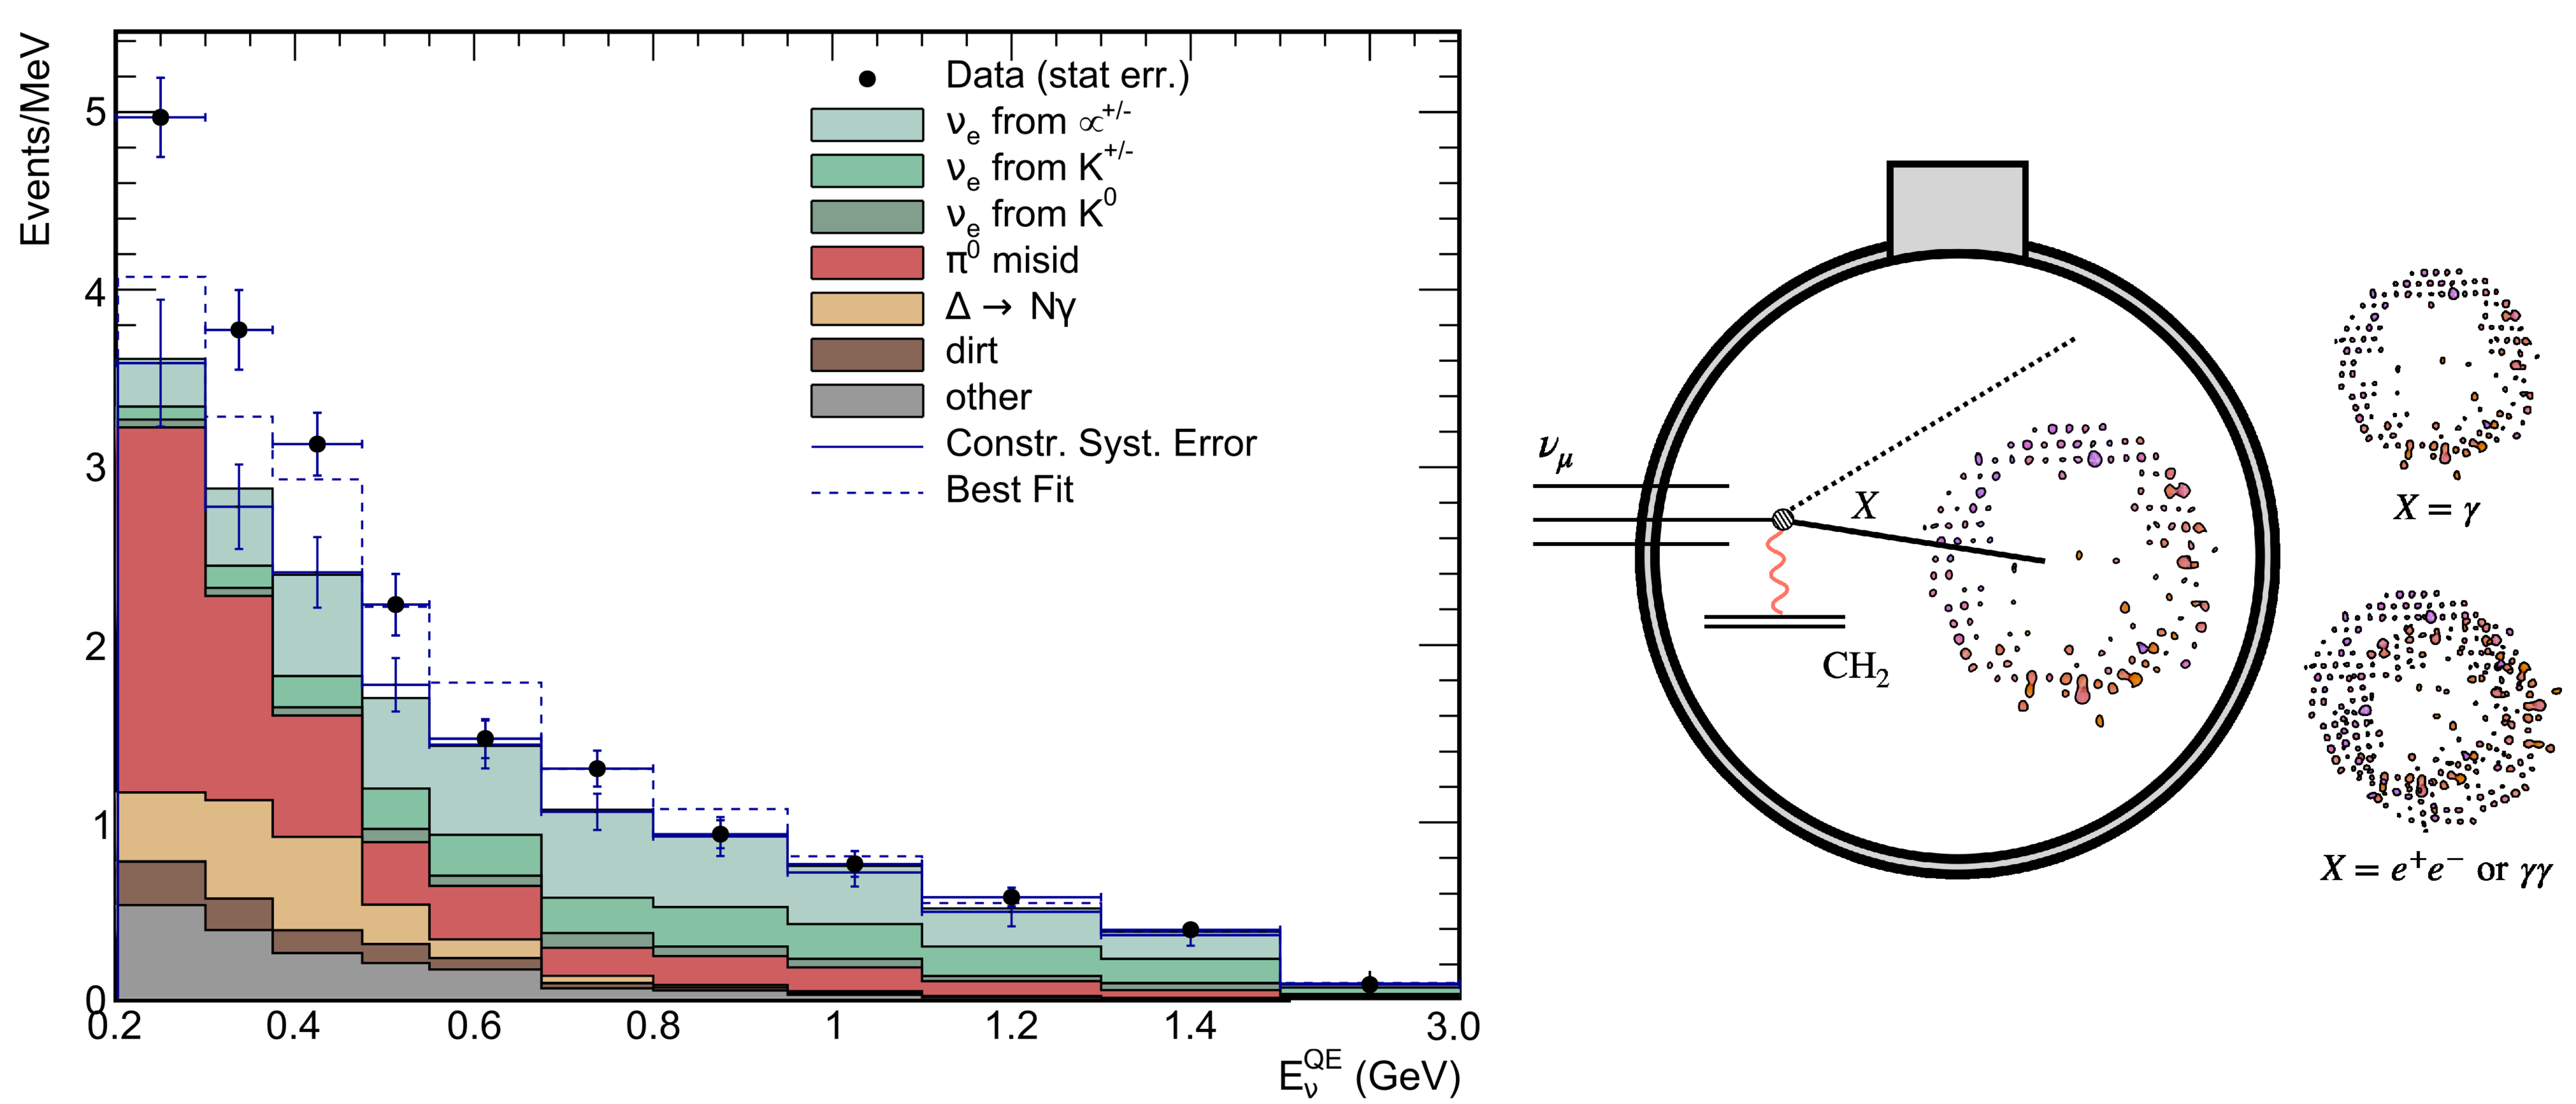
\includegraphics[width=0.9\linewidth]{anomalies/miniboone_results.pdf}
    \caption[MiniBooNE detector and results]{(left) Neutrino energy distribution of $\PGne$CC QE events recorded by the MiniBooNE detector with data acquisition in neutrino mode. The dashed histogram shows the best fit to the neutrino-mode data assuming two-neutrino oscillations. (right) An example of the typical interactions visible inside the detector, with different signatures for different final state interactions.}
    \label{fig:MiniBooNE}
\end{figure}

\paragraph{Reactor antineutrino experiments} Reactor antineutrinos played a central role in establishing the three-flavour oscillation paradigm. In the simplest sterile neutrino picture (more details are provided in \autoref{sec:sterile_theory}) where one additional sterile neutrino is assumed ($3+1$ scheme), $\PGne$ disappearance in neutrinos from reactors should be possible, with detectors placed $<\SI{100}{m}$ from the neutrino source. In such experiments, respectivelly located at ILL-Grenoble, Goesgen, Rovno, Krasnoyarsk, Savannah River and Bugey \cite{mentionReactorAntineutrinoAnomaly2011}, the measured rate of $\PGne$ was in reasonable agreement with that predicted from the reactor antineutrino spectra, though slightly lower than expected, with the measured/expected ratio at $R=\num{0.976+-.024}$, representing a $2.7\sigma$ deviation from the prediction. This is known as the ``reactor antineutrino anomaly'' (RAA). The additional measurements by the long-baseline detectors KamLAND and CHOOZ (the CHOOZ experiment is consistent with no oscillation) provided a stricter lower result of such ratio, at $R=\num{0.943 +- 0.023}$, deviating from the unity with a statistical significance of $\SI{98.6}{\percent}$ CL. 

\paragraph{Radioactive sources experiments} Radioactive sources are often used for the calibration of different types of detectors. This was the case for both the GALLEX and SAGE solar neutrinos detectors. Such experiments employed natural radioactive sources, either $^{51}$Cr or $^{37}$Ar, which both produce electron neutrinos through electron capture processes \begin{align}
    \Pem + {}^{51}\mathrm{Cr} &\to {}^{51}\mathrm{V} + \PGne, && \text{(GALLEX)}\\
    \Pem + {}^{37}\mathrm{Ar} &\to {}^{37}\mathrm{Cl} + \PGne, && \text{(GALLEX, SAGE)}
\end{align} placed inside the detector, to calibrate the flux of electron neutrinos with respect to the rate of electron capture processes $\PGne + {}^{71}\mathrm{Ga} \to {}^{71}\mathrm{Ge} + \Pem$ observed. Both experiments, during the detector calibration, observed a deficit of counts with respect to the well-know activities of the sources, with average ratios $\overline R$ ranging from $\numrange{0.703 +- 0.078}{0.844 +- 0.031}$ \cite{giuntiGalliumAnomalyCritical2022}, showing a statistical significance of $2.2\sigma$. A dedicated experiment was later planned, the Baksan Experiment on Sterile Transitions (BEST) to test such results, and a larger deficit was observed. Combining all radiochemical measurements increased significance of the so called ``Gallium Anomaly'' (GA) to $\sim4\sigma$, with $\overline{R} = \num{0.80+-0.04}$ \cite{elliottGalliumAnomaly2023}. 

\subsection{The sterile neutrino hypothesis} \label{sec:sterile_theory}

The picture presented so far seems to hint, from multiple perspectives, at the possibility of an additional sterile neutrino scenario. This requires the introduction of a fourth sterile --- i.e. not weakly interacting --- neutrino state, taking part in short baseline oscillation, with a mass splitting of $\Delta m^2 {\sim} \mathcal{O}(\SI{1}{eV^2})$. The need for this state to be ``sterile'' is required to minimally extend the SM, since the introduction of a massive weakly interacting particle with $m<m_\PZ/2$ would not be possible. 

The most general approach to introducing sterile particle content in the leptonic sector would be to add $N$ sterile neutrinos and consider a $(3+N)\times(3+N)$ PMNS matrix. This is the most general way of introducing sterile neutrinos in the model, but to keep the number of parameters as small as possible (occam razor), it is effectively interesting to look at a ``simpler'' one, where only one additional sterile family is introduced. This $3+1$ paradigm, which is what will be considered in the following paragraphs, requires the introduction of a sterile state $\PGns$, and a basis of four massive neutrinos $\PGn_1, \dots, \PGn_4$, with the additional assumption that the fraction of $\PGns$ is extremely small for the first three mass eigenstates and near \SI{100}{\percent} for the fourth, as illustrated in \autoref{fig:ordering_NO_sterile}. 

\begin{figure}
    \centering
    \begin{tikzpicture}[
        nue/.style={fill=Red!70!white},
        numu/.style={fill=ForestGreen!65!white},
        nutau/.style={fill=MidnightBlue!65!white},
        nusterile/.style={fill=Gray!35!white},
        scale=0.75
    ]

        %%%%%%%%%%%%%%%%%%%%%%%%%%%%%%%%%%%%%%%%%%%%%%%%%%%%%%%%%%%%%%%%%%%%%%%%%%%%%%%%
        %%%%%% NORMAL MASS ORDERING %%%%%%%%%%%%%%%%%%%%%%%%%%%%%%%%%%%%%%%%%%%%%%%%%%%%
        %%%%%%%%%%%%%%%%%%%%%%%%%%%%%%%%%%%%%%%%%%%%%%%%%%%%%%%%%%%%%%%%%%%%%%%%%%%%%%%%

        \node[text centered] at (-3,4.5) {Normal ordering};
        \node[text centered] at (-0.25,4.5) {$\delta_\mathrm{CP}$};

        \node[text centered] at (-5.5, 3.75)  {$\PGn_4$};
        \node[text centered] at (-5.5, -.75)  {$\PGn_3$};
        \node[text centered] at (-5.5, -3.75) {$\PGn_2$};
        \node[text centered] at (-5.5, -4.75) {$\PGn_1$};

        \fill[nusterile] (-1,4) -- (-5,4) -- (-5,3.5) -- (-1,3.5) -- cycle;
        \fill[nue] (-.9,4) -- (-1,4) -- (-1,3.5) -- (-.9,3.5) -- cycle;
        \fill[numu] (-.825,4) -- (-.9,4) -- (-.9,3.5) -- (-.825,3.5) -- cycle;
        \fill[nutau] (-.75,4) -- (-.825,4) -- (-.825,3.5) -- (-.75,3.5) -- cycle;

        \draw[black] (-5,4) rectangle (-0.75,3.5);

        \node[text centered] at (-.25, 4) {\small$\pi$};
        \node[text centered] at (-.25, 3.5) {\small 0};
        
        \fill[nusterile] (-0.75,-.5) -- (-1,-.5) -- (-1,-1) -- (-.75,-1) -- cycle;
        \fill[nue] (-5,-.5) -- (-4.75,-.5) -- (-4.75,-1) -- (-5,-1) -- cycle;
        \fill[numu] (-4.75,-.5) -- (-3.,-.5) -- (-3.,-1) -- (-4.75,-1) -- cycle;
        \fill[nutau] (-3.,-.5) -- (-1,-.5) -- (-1,-1) -- (-3.,-1) -- cycle;

        \draw[black] (-5,-.5) rectangle (-.75,-1);

        \node[text centered] at (-.25, -.5) {\small$\pi$};
        \node[text centered] at (-.25, -1) {\small 0};

        \fill[nusterile] (-0.75,-3.5) -- (-1,-3.5) -- (-1,-4) -- (-.75,-4) -- cycle;
        \fill[nue] (-5,-3.5) -- (-4.,-3.5) -- (-4.,-4) -- (-5,-4) -- cycle;
        \fill[numu] (-4.,-3.5) -- (-2.15,-3.5) -- (-3,-4) -- (-4,-4) -- cycle;
        \fill[nutau] (-2.15,-3.5) -- (-1,-3.5) -- (-1,-4) -- (-3.,-4) -- cycle;

        \draw[black] (-5,-3.5) rectangle (-.75,-4);

        \node[text centered] at (-.25, -3.5) {\small$\pi$};
        \node[text centered] at (-.25, -4) {\small 0};

        \fill[nusterile] (-0.75,-4.5) -- (-1,-4.5) -- (-1,-5) -- (-.75,-5) -- cycle;
        \fill[nue] (-5,-4.5) -- (-2.575,-4.5) -- (-2.575,-5) -- (-5,-5) -- cycle;
        \fill[numu] (-2.575,-4.5) -- (-2.2,-4.5) -- (-1.25,-5) -- (-2.575,-5) -- cycle;
        \fill[nutau] (-2.2,-4.5) -- (-1,-4.5) -- (-1,-5) -- (-1.25,-5) -- cycle;

        \draw[black] (-5,-4.5) rectangle (-.75,-5);

        \node[text centered] at (-.25, -4.5) {\small$\pi$};
        \node[text centered] at (-.25, -5) {\small 0};

        \draw[gray, line width=1mm] (-6.25, -4.85) -- (-6.25, -3.65);
        \draw[gray, line width=1mm] (-6, -.65) -- (-6, -3.85);

        \draw[gray, line width=1mm] (-6.25, -0.85) -- (-6.25, 0.65);
        \draw[gray, line width=1mm, dotted] (-6.25, 0.65) -- (-6.25, 2.15);
        \draw[gray, line width=1mm] (-6.25, 2.15) -- (-6.25, 3.65);

        \node[] at (-8.35, -4.25) {
            \begin{minipage}{2cm}
                \raggedleft
                Solar\\
                $\sim \SI{e-5}{eV^2}$
            \end{minipage}
        };

        \node[] at (-8.35, -2.25) {
            \begin{minipage}{2cm}
                \raggedleft
                Atmospheric\\
                $\sim \SI{e-3}{eV^2}$
            \end{minipage}
        };

        \node[] at (-8.35, 1.5) {
            \begin{minipage}{2cm}
                \raggedleft
                Sterile\\
                $\sim \SI{1}{eV^2}$
            \end{minipage}
        };

        \draw[-*, Red!65!black, shorten >=-2pt] (-4, -5.5) node[below, text centered] {$\PGne$} -- (-4, -5);
        \draw[-*, ForestGreen!65!black, shorten >=-2pt] (-2, -5.5) node[below, text centered] {$\PGnGm$} -- (-2, -5);
        \draw[-*, MidnightBlue!65!black, shorten >=-2pt] (-1.15, -5.5) node[below, text centered] {$\PGnGt$} -- (-1.15, -5);

        \draw[-*, Gray!65!black, shorten >=-2pt] (-.85, -3) node[above, text centered] {$\PGns$} -- (-.85, -3.5);
    \end{tikzpicture}
    \caption[Neutrino mass ordering with the sterile state]{Representation of mass ordering, mixing, and splitting in the $3+1$ scenario. Normal ordering is assumed for the other three massive states. Expanded from \cite{menaUnifiedGraphicalSummary2004}.}
    \label{fig:ordering_NO_sterile}
\end{figure}

From the experimental evidence we can assign $\Delta m^2_{4\ell} {\sim} \mathcal O (\SI{1}{eV^2})$, and since it is greater than the atmospheric and the solar mass splitting, the oscillation probability can be computed neglecting such terms --- the so-called short-baseline approximation ---, thereby giving rise to a new two-flavour oscillation probability that holds at small distances \begin{align}
    P(\PGn_\ell \rightarrow \PGn_\ell) &\simeq 1 - 4 |U_{\ell4}|^2 (1 - |U_{\ell4}|^2) \sin^2 \left( \frac{\Delta m^2_{41} L}{4 E_\PGn} \right) \nonumber \\
    &\qquad\qquad\qquad\equiv 1 - \sin^2 (2\theta_{\ell\ell}) \sin^2 \left( \frac{\Delta m^2_{41} L}{4 E_\PGn} \right),\quad \ell = \Pe, \PGm \label{eq:2body_oscillation_sterile_disapp}\\
    P(\PGnGm \rightarrow \PGne) &\simeq 4 |U_{\PGm4}|^2 |U_{\Pe4}|^2 \sin^2 \left( \frac{\Delta m^2_{41} L}{4 E_\PGn} \right) \nonumber \\
    &\qquad\qquad\qquad\equiv \sin^2 (2\theta_{\PGm\Pe}) \sin^2 \left( \frac{\Delta m^2_{41} L}{4 E_\PGn} \right). \label{eq:2body_oscillation_sterile_app}
\end{align} where the first equation can be either the disappearance probability of electron or muon neutrinos, and the second controls the appearance probability of electron neutrinos from a beam of pure muon neutrinos. The ``effective'' mixing angles $\theta_{\alpha\beta}$ are directly correlated with the elements of the extended PMNS matrix in the hypothesis of a $3+1$ oscillation scenario. 

\subsection{Experimental status and future perspectives}

The experimental landscape of the sterile neutrino searches has broadened, over the years, with even more experiments adding limits to the phase space. To this day, no definitive picture has completely proved or discarded the existence of this fourth sterile neutrino state. 

Different experiments can be distinguished based on the technique, target channel and the final result (evidence of a signal or data fit compatible  with the null hypothesis). The experimental landscape can be classified by the channel where it is performing its research and by the result it found (i.e. \emph{did it find any anomaly?}).

One of the most significant experimental anomalies comes from the LNSD experiment. The MiniBooNE LEE in $\PGne$-appearance analysis is compatible with the results of the LNSD experiment, yet still preferring a higher mixing angle $\sin^22\theta {\sim} \num{0.807}$ and smaller mass splitting $\Delta m^2 \simeq \SI{0.043}{eV^2}$, compared to that of LNSD. It is interesting to note (for reference, see \autoref{fig:MiniBooNE}) that the $3+1$ sterile scenario did not fully explain the excess seen by the MiniBooNE experiment. 

Similar to the LSND experiment was the KARMEN experiment, which, however, did not find any signature of $\PAGnGm\to\PAGne$ oscillations \cite{collaborationUpperLimitsNeutrino2002}. The KARMEN experiment operated in similar conditions to those of the LSND experiment, but at a shorter baseline of \SI{17.7}{\m}, thereby restricting its allowed parameter space. This posed some limits to the allowed parameter space compared to the one explored by the LSND experiment, thus not excluding its claim. Other ``null-result'' experiments were performed following the results of LSND and MiniBooNE, including the NOMAD experiment, which operated at a baseline of about \SI{620}{m} from the source of neutrinos, produced using the SPS accelerator at CERN and with energies of ${\sim}\SI{20}{GeV}$. It excluded at \SI{90}{\percent} CL the higher mass splitting values, adding the constraints $\Delta m^2 < \SI{0.4}{eV^2}$ (with maximal mixing) and $\sin^22\theta < \num{1.4e-3}$ for large mass splittings \cite{collaborationSearchNumu>nueOscillations2003}. MiniBooNE LEE was explored by many similar experiments; particularly interesting is the MicroBooNE experiment, MiniBooNE's immediate successor, collecting data from BNB upstream of MiniBooNE at \SI{472}{m} distance from the neutrino source. The technology is that of the Liquid Argon Time Projection Chamber \cite{rubbiaLiquidArgonTime1977}, which will be described in detail in \autoref{chap:icarus_detector}. The MicroBooNE experiment studied the individual channels of teh MiniBooNE backgrounds to see wheter the LEE could be created by a mismodeling of the backgrounds or wheter an oscillatory effect was really observed. Looking at muliple final state topologies in the $\PGne$ channel, MicroBooNE data indicated that no LEE-like signal was evident, and that background seen by MiniBooNE are coherent with the unoscillated hypotesis \cite{collaborationSearchExcessElectron2022}. However, these findings were proved to not be definitive \cite{arguellesMicroBooNE$n_e$Interpretation2022} since the exclusion area of the MicroBooNE experiment could not rule out the allowed parameter space of the best fit of the MiniBooNE experiment. 

At long baseline multiple experiments also investigated LNSD and MiniBooNE LEE anomalies. This is, for example, the case of the ICARUS LNGS run and OPERA (CNGS1/2) experiments, collecting neutrinos produced from the S$\Pp\PAp$S in the CNGS beam at an energy of ${\sim} \SI{17}{GeV}$ and placed at baselines of \SI{730}{km}. Both the ICARUS \cite{antonelloSearchAnomaliesNeappearance2013, antonelloConclusiveConsiderationsComparison2015} and the OPERA \cite{agafonovaNewResultsNm2013} experiments results excluded much of the parameter space of the MiniBooNE experiment, especially in the high mixing angle region, showing \begin{align}
    \sin^22\theta &< \num{6.8e-3}\ (\num{1.52e-2})\ \text{at \SI{90}{\percent} (\SI{99}{\percent}) CL,} && \text{(ICARUS)}\\
    \sin^22\theta &< \num{7.2e-3}\ \text{at \SI{90}{\percent} CL.} && \text{(OPERA)}
\end{align}

A relevant tension is also found comparing results from very short baseline reactor experiments. The target searches are excess or deficits in the electron antineutrino flux, so it is clear that a correct evaluation of the expected flux of antineutrinos is key for such measurement. However, recent theoretical models are not in agreement with the experimental results, thereby affecting the systematic uncertainties related to the oscillation measurements. Reactor experiments are mostly not sensitive to the spectrum of energies but are considered ``rate'' experiments, counting the overall excess of the flux, or ``spectral'' experiments, looking at the energy --- or $E/L$ --- spectrum. Particularly relevant are the results of the Bugey \cite{declaisSearchNeutrinoOscillations1995}, NEOS \cite{koSterileNeutrinoSearch2017}, PROSPECT \cite{andriamiradoImprovedShortBaselineNeutrino2020} and STEREO \cite{almazanSTEREONeutrinoSpectrum2023} experiments, which found no evidence of oscillation. NEOS was followed by the RENO experiment. The two experiments detected neutrinos produced by the same source thereby, suppressing many of the uncertainties in the flux model. The results of these experiments narrowed the parameter space with respect to the previous results \cite{atifSearchSterileNeutrino2022}. 

In the reactor neutrino experiment landscape, an interesting result is that of the Neutrino-4 experiment. This experiment measures electron antineutrinos from a nuclear reactor SM-3 in Dimitrovgrad, Russia, using a movable detector with the ability to investigate the \qtyrange{6}{10}{m} range of baseline distances from the reactor. This experiment reported evidence of $L/E \simeq \qtyrange{1}{3}{m/MeV}$ oscillation, with a sensitivity of roughly $3\sigma$. This result is in great agreement with GA experiments such as GALLEX and SAGE. This is the sole case where this happens, since most of the RAA experiments are in tension with GA experiments \cite{maltoniEVSterileNeutrinos2024}. When combined with GALLEX, SAGE and BEST its statistical significance rises to $5.8\sigma$ \cite{serebrovResultNeutrino4Experiment2023}. The result of the Neutrino-4 experiment fits well the $3+1$ scenario, leading to a mass splitting of $\Delta m^2_{41} = \mathrm{7.30\pm0.13\ (stat) \pm 1.16\ (syst)}\ \si{eV^2} = \SI{7.30+-1.17}{eV^2}$ and an amplitude of $\sin^22\theta = \num{0.36\pm0.12}\mathrm{\ (stat.)}$. 

As previosly mentioned, GA experiment results are in tension with most of the other experimental searches as they require a greater mixing angle. This anomaly leads to a best-fit point $(\Delta m^2, \sin^22\theta) \simeq (\SI{1.25}{eV^2}, \num{0.32})$ \cite{giuntiGalliumAnomalyCritical2022}. The overlap with the allowed regions of the LNSD and MiniBooNE LEE is negligible, and the overlap with RAA is possible with $\sin^22\theta\sim0.2$. 

Other experimental searches focuse on the $\PGnGm$-disappearance and $\PGne$-appearance channels. These channels have been explored by NOvA \cite{collaborationSearchActivesterileNeutrino2017}, MINOS and MINOS$+$ \cite{adamsonSearchSterileNeutrinos2019}. Additional searches have also been performed with data from the IceCube detector, and interesting results will come from the JUNO neutrino experiment \cite{dentlerUpdatedGlobalAnalysis2018}, which is now collecting its first data \cite{Yu:2025ygh}. 

\autoref{fig:all_experimental_searches} shows a summary of all the experiments that provided exclusion areas in the parameter space, with the baseline at which they are detecting neutrinos and their energy range superimposed to the oscillation maxima in the hypothesis of a two-flavour oscillation scenario.

In this very complicated picture stands the Short-Baseline-Neutrino program \cite{acciarriProposalThreeDetector2015}, to which the next chapter is briefly devoted. In \autoref{fig:sensitivity_plots} are shown the updated allowed and excluded parameter regions from the combination of the multiple ocillation channels and multiple experimental inputs. This experiment will probe the sterile neutrino scenario with increased sensitivity up to $5\sigma$, exploiting a two-detector experimental search in both the $\PGne$-appearance and $\PGnGm$-disappearance channels. 

\begin{sidewaysfigure}
    \centering

    \subfloat[]{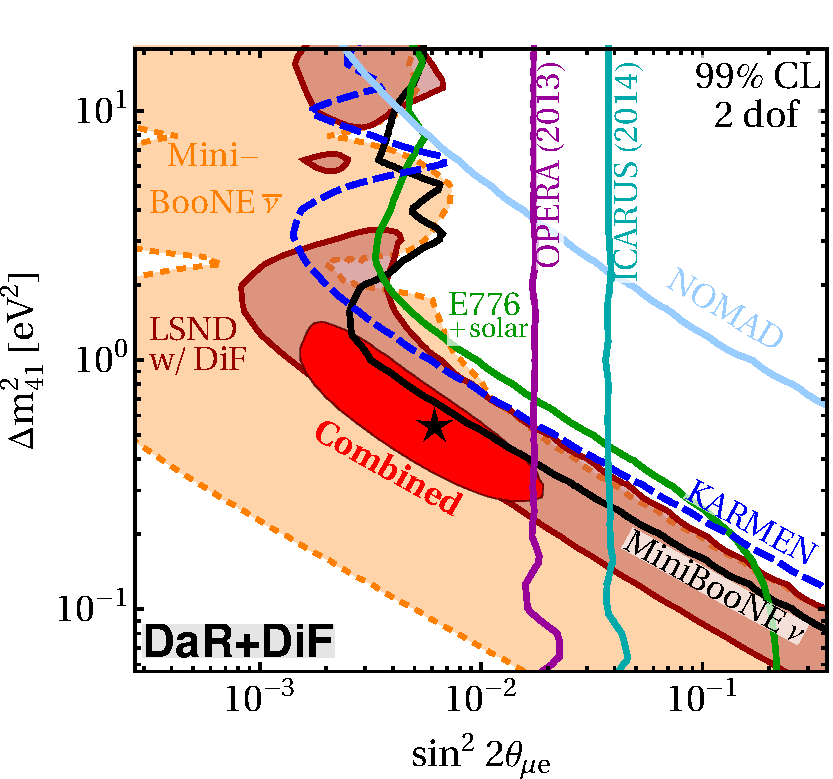
\includegraphics[height=8cm, trim={1cm  0 0 0}]{anomalies/DM41sin22mueDiF.pdf}\label{fig:DM41sin22mueDiF}}
    \hspace{1cm}
    \subfloat[]{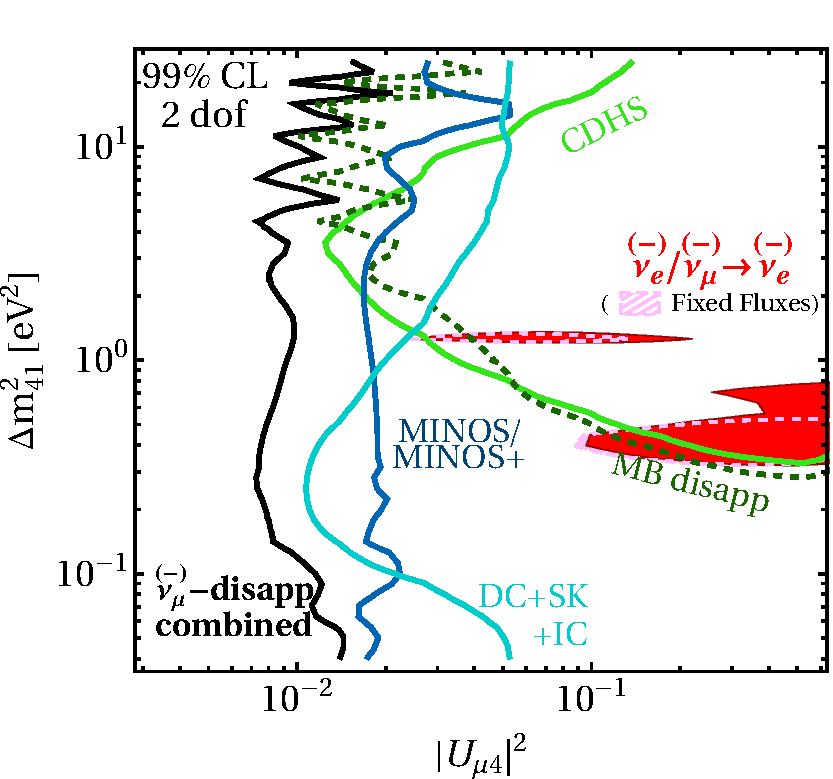
\includegraphics[height=8cm, trim={0.75cm  0 0 0}, clip]{anomalies/dm41Um4.pdf}\label{fig:dm41Um4}}
    \caption[Parameter spaces in both the $\PGne$ appearance and $\PGnGm$ disappearance channels]{\ref{sub@fig:DM41sin22mueDiF} Constraints on short-baseline $\PGnGm\to\PGne$ and $\PAGnGm\to\PAGne$ oscillations from the present experimental results in the presence of sterile neutrinos in $3 + 1$ scenarios. \ref{sub@fig:dm41Um4} Constraints on the $3 + 1$ scenario from $\PGnGm/\PAGnGm$ disappearance. Picture taken from \cite{dentlerUpdatedGlobalAnalysis2018}.}
    \label{fig:sensitivity_plots}
\end{sidewaysfigure}

\begin{sidewaysfigure}
    \centering
    \subfloat[]{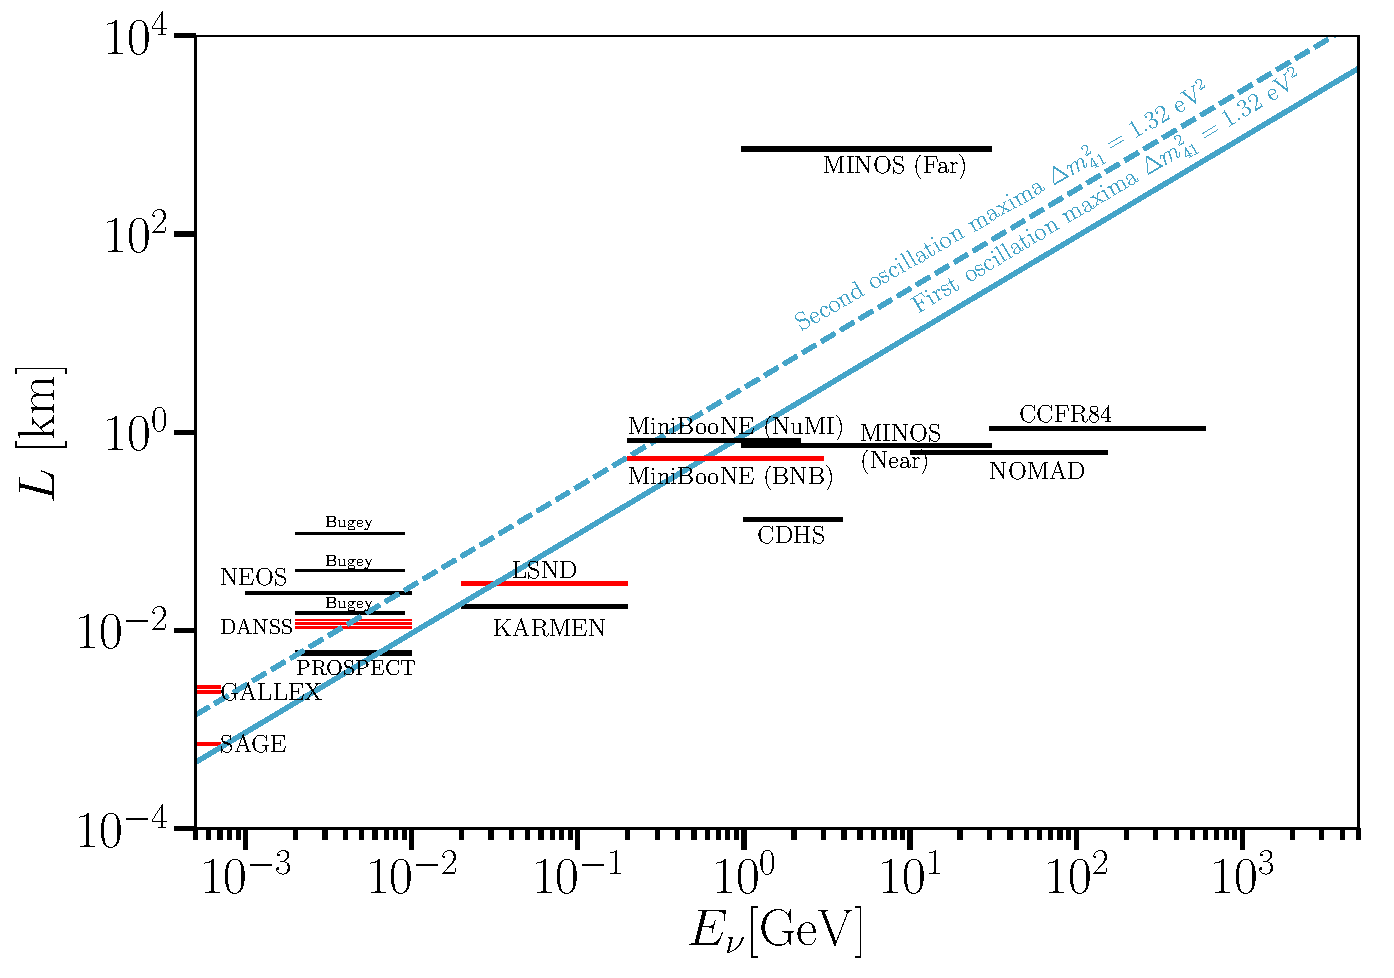
\includegraphics[width=0.475\linewidth]{anomalies/all-experiments.pdf}\label{fig:all_exp_A}}
    \subfloat[]{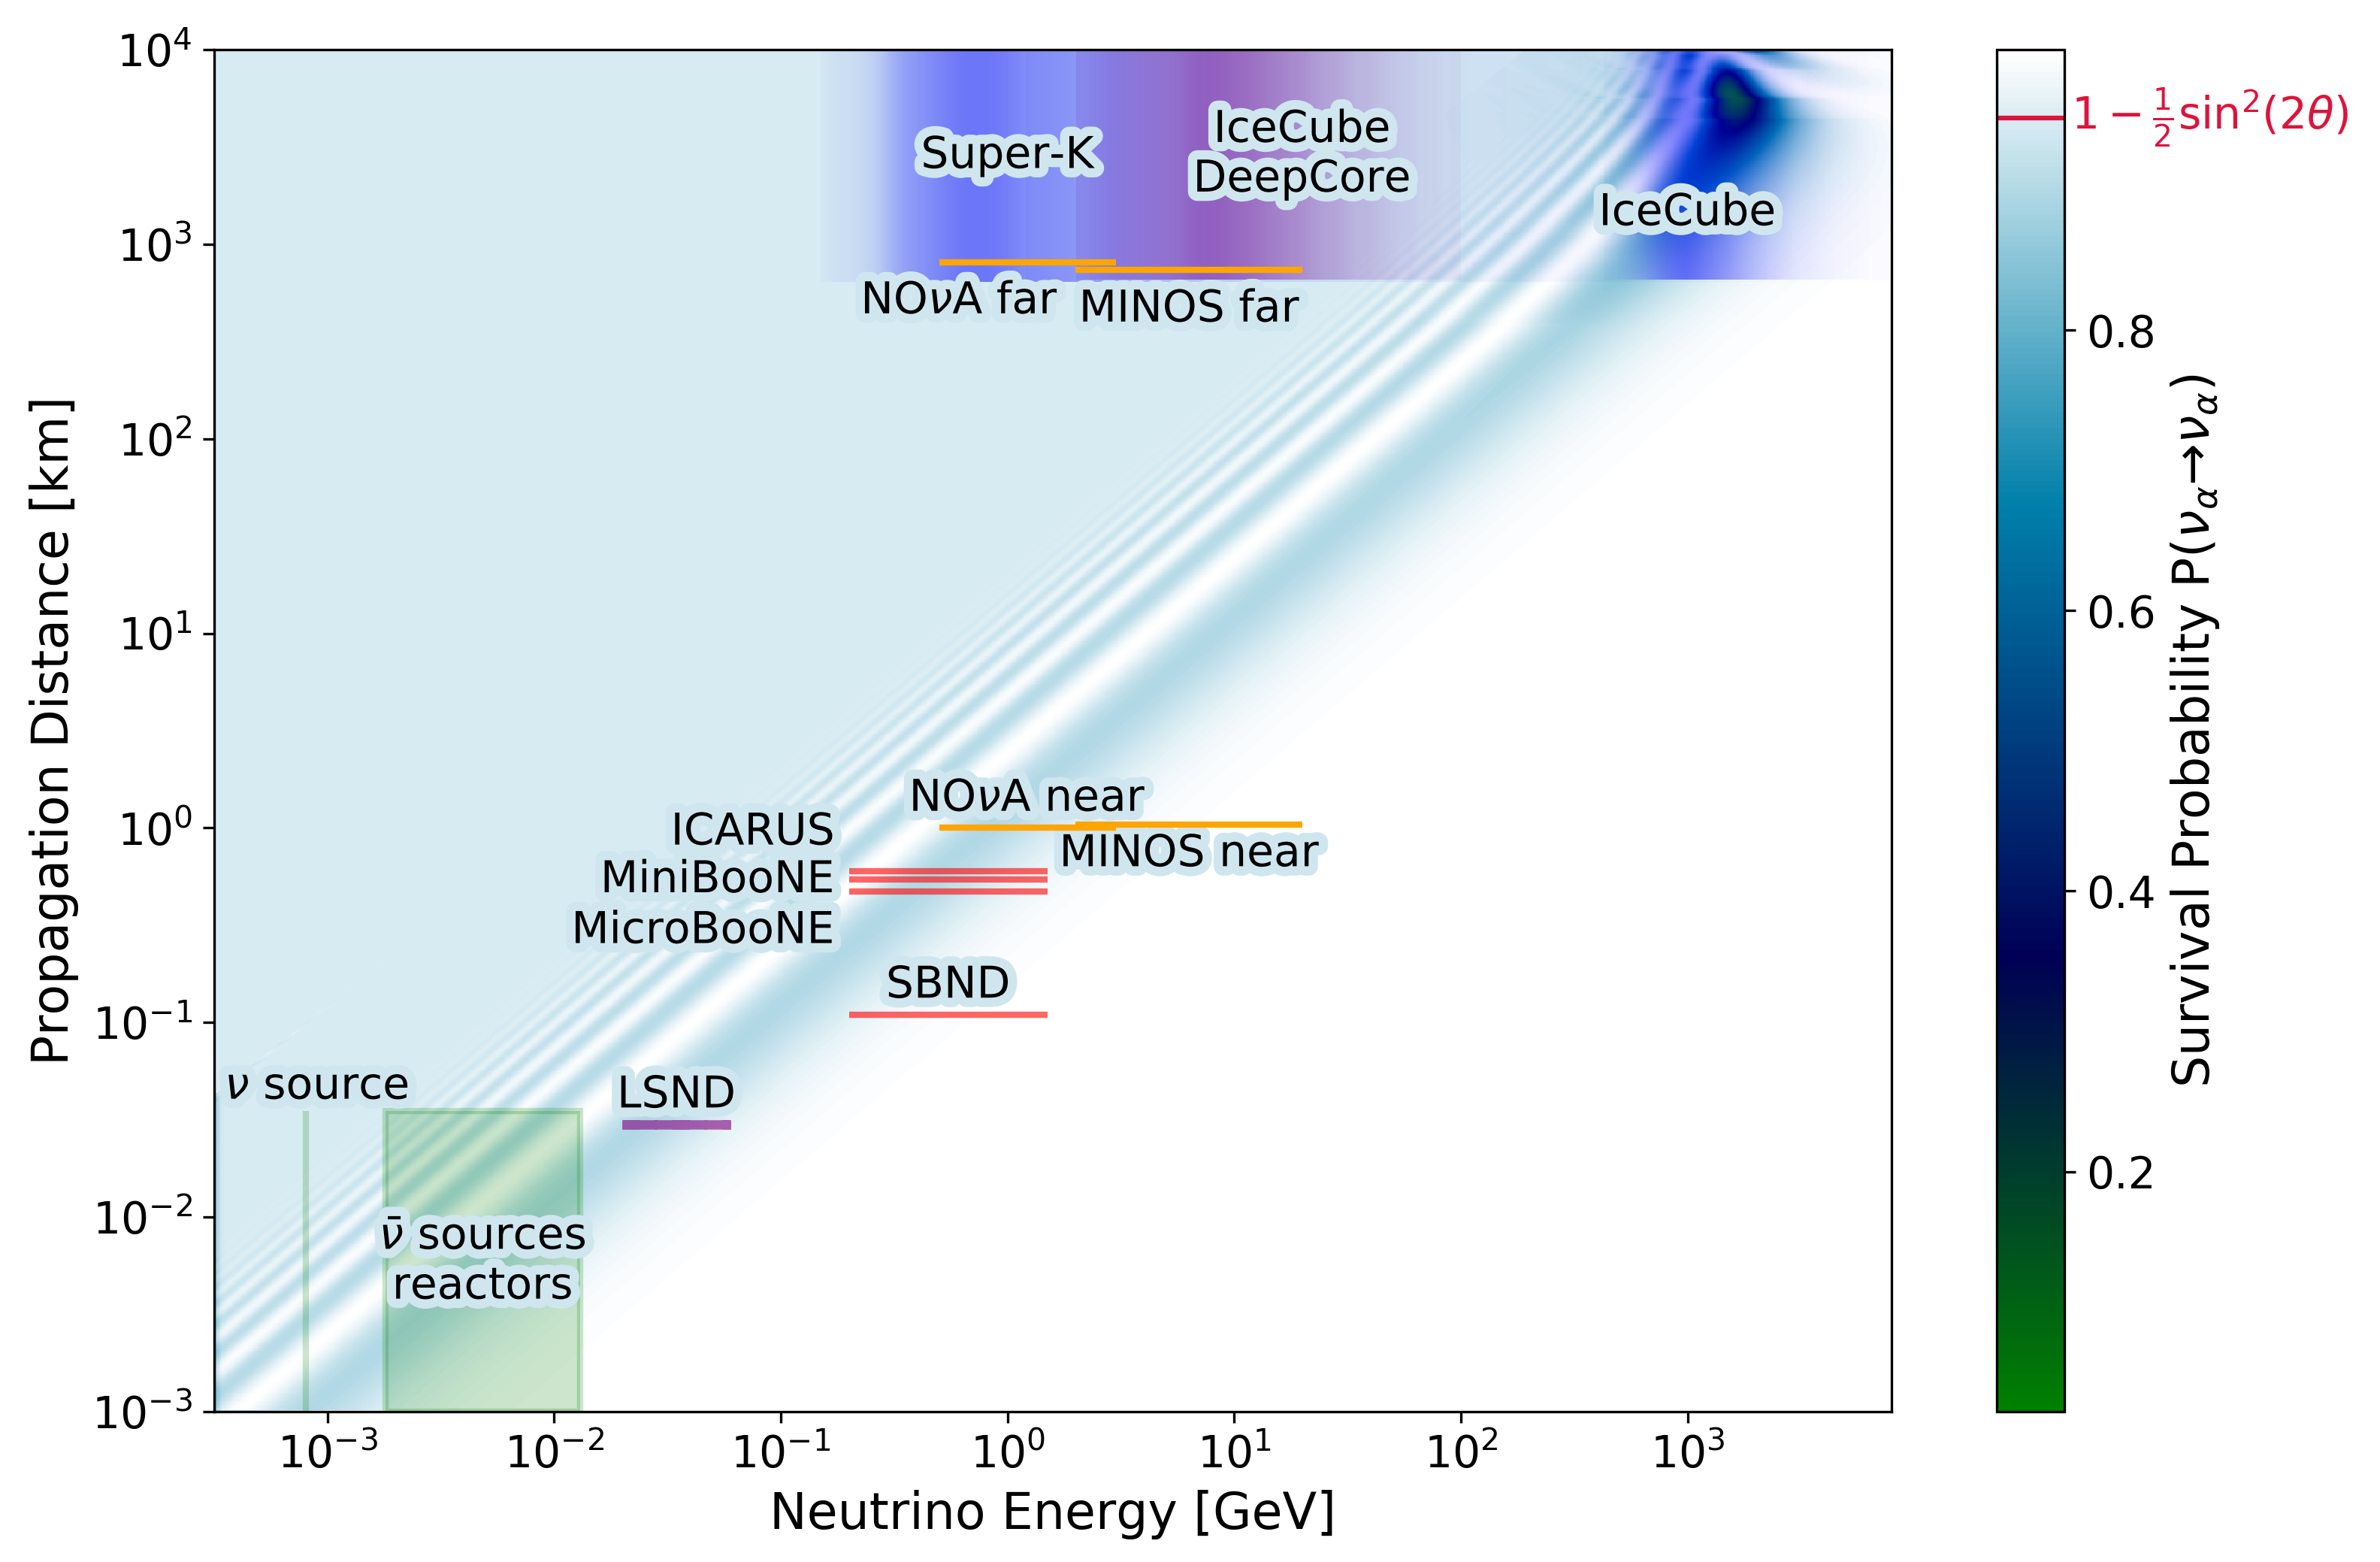
\includegraphics[width=0.525\linewidth]{anomalies/sterile_osc_overview.png}\label{fig:all_exp_B}}
    \caption[Status of the global experimental searches]{\ref{sub@fig:all_exp_A} (Incomplete) list of experiments searching for sterile neutrino oscillations, with baseline and energy range explored highlighted. The position of the first and second oscillation maxima for $\Delta m^2 = \SI{1.32}{eV^2}$ is also highlighted. Experiments with results indicating a $>2\sigma$ preference for the $3+1$ mixing scheme are shown in red. Picture taken from \cite{diazWhereAreWe2020a}. \ref{sub@fig:all_exp_B} Other, mostly new generation, experiments searching for sterile neutrino oscillations. The plot additionally show through shaded areas the survivl probability $P(\HepParticle{\PGn}{\ell}{}\to\HepParticle{\PGn}{\ell}{})$. Picture taken from \cite{boserStatusLightSterile2020}. }
    \label{fig:all_experimental_searches}
\end{sidewaysfigure}

% FINAL CITATION
\nocite{triozziStudyTriggerSystem, arteroponsStudyReconstructionNuMuCC}